% =====================================================================
%  Rapport de stage PFE — Gestion des agences bancaires (BTK)
%  Esprit School of Business — Licence Business Computing / BI
%  Compilation : pdflatex main ; bibtex main ; pdflatex main ; pdflatex main
% =====================================================================
\documentclass[a4paper,12pt,oneside]{report}

% ---- Encodage & langue ----
\usepackage[T1]{fontenc}
\usepackage[utf8]{inputenc}
\usepackage{newtxtext,newtxmath}     % Times New Roman (corps + maths)
\usepackage[french]{babel}
\usepackage{csquotes}

% ---- Mise en page (charte : marges 2,5 cm, interligne 1,15) ----
\usepackage[a4paper,margin=2.5cm]{geometry}
\usepackage{setspace}
\setstretch{1.15}
\usepackage{microtype}
% Tolérance de césure : évite les débordements dans la marge dus aux longs
% identifiants de code (\texttt) non sécables, en autorisant un léger relâchement.
\tolerance=2000
\emergencystretch=3em

% ---- Graphiques, couleurs, tableaux ----
\usepackage{graphicx}
\graphicspath{{images/}{diagrams/}}
\usepackage{xcolor}
\definecolor{btkblue}{HTML}{14507A}
\definecolor{btklight}{HTML}{1B6CA8}
\usepackage{booktabs}
\usepackage{array}
\usepackage{longtable}
\usepackage{tabularx}
\usepackage{multirow}
\usepackage{enumitem}
\usepackage{ragged2e}
% Colonnes X en alignement « ragged right » : évite l'étirement et les
% débordements dus aux identifiants de code (\texttt) dans les tableaux.
\renewcommand{\tabularxcolumn}[1]{>{\RaggedRight\arraybackslash}p{#1}}

% ---- Légendes : « Figure 1.1 – ... » (numérotation par chapitre native) ----
\usepackage{caption}
\captionsetup{labelsep=endash,font=small,labelfont=bf}

% ---- En-têtes / pieds : numéro de page en bas à droite ----
\usepackage{fancyhdr}
\pagestyle{fancy}
\fancyhf{}
\fancyfoot[R]{\thepage}
\renewcommand{\headrulewidth}{0pt}
\renewcommand{\footrulewidth}{0pt}
\fancypagestyle{plain}{\fancyhf{}\fancyfoot[R]{\thepage}%
  \renewcommand{\headrulewidth}{0pt}}

% Numéroter et lister jusqu'aux sous-sous-sections (ex. 1.4.3.1)
\setcounter{secnumdepth}{3}
\setcounter{tocdepth}{3}

% ---- Style des titres de chapitre ----
\usepackage{titlesec}
\titleformat{\chapter}[display]
  {\normalfont\huge\bfseries\color{btkblue}}
  {\chaptertitlename\ \thechapter}{16pt}{\Huge}
\titlespacing*{\chapter}{0pt}{0pt}{24pt}

% ---- Listings (extraits de code Python de la chaîne ETL) ----
\usepackage{listings}
\lstdefinestyle{pycode}{
  language=Python,
  basicstyle=\ttfamily\footnotesize,
  keywordstyle=\color{btkblue}\bfseries,
  commentstyle=\color{gray}\itshape,
  stringstyle=\color{btklight},
  numbers=left, numberstyle=\tiny\color{gray}, numbersep=8pt,
  frame=single, rulecolor=\color{btkblue!40},
  backgroundcolor=\color{btkblue!4},
  breaklines=true, showstringspaces=false, columns=fullflexible,
  literate={é}{{\'e}}1 {è}{{\`e}}1 {à}{{\`a}}1 {ê}{{\^e}}1 {î}{{\^\i}}1 {ç}{{\c c}}1
}

% ---- Fiche de description textuelle d'un cas d'utilisation ----
% #1 label, #2 titre, #3 objectif, #4 acteur, #5 pré-condition, #6 post-condition, #7 scénario
\newcommand{\cudesc}[7]{%
\begin{table}[htbp]\centering
\caption{Description textuelle du cas d'utilisation « #2 »}\label{#1}
\renewcommand{\arraystretch}{1.3}
\begin{tabularx}{\textwidth}{>{\bfseries}p{3.2cm}X}
\toprule
\textmd{\textbf{Titre}} & #2\\
\midrule
Objectif & #3\\
Acteur & #4\\
Pré-condition & #5\\
Post-condition & #6\\
Scénario nominal & #7\\
\bottomrule
\end{tabularx}
\end{table}}

% ---- Liens & références croisées ----
\usepackage[hidelinks]{hyperref}
\usepackage{cleveref}
\usepackage{pdflscape}   % pages en paysage (rotation dans le PDF)

\begin{document}

% ============================ PAGE DE GARDE ===========================
% ============================ PAGE DE GARDE ===========================
% Structure alignée sur le modèle ESB (rapport de stage)
\begin{titlepage}
\centering
\thispagestyle{empty}
\definecolor{esred}{HTML}{000000}  % tout en noir (charte demandée)

% ---- En-tête : établissement ----
{\large\bfseries École Supérieure Privée de Management de Tunis}\\[0.15cm]
{\large\bfseries Esprit School of Business}\\[1.1cm]

% ---- Logos : ESB (gauche) et BTK (droite) ----
\begin{minipage}[c]{0.48\textwidth}\centering
  
\includegraphics[height=2.5cm,keepaspectratio]{logo_esb.png}
\end{minipage}\hfill
\begin{minipage}[c]{0.48\textwidth}\centering
  
\includegraphics[height=2.5cm,keepaspectratio]{logo_btk.png}
\end{minipage}\\[1.3cm]

% ---- Titre principal ----
{\fontsize{40}{44}\selectfont\bfseries\color{esred} RAPPORT DE STAGE}\\[0.2cm]
{\color{esred}\rule{\textwidth}{1.4pt}}\\[0.55cm]

{\large En vue de l'obtention du diplôme de Licence en Business Computing}\\[0.45cm]
{\large\bfseries Parcours Business Intelligence}\\[0.25cm]
{\color{esred}\rule{0.72\textwidth}{1pt}}\\[0.9cm]

% ---- Auteur (pas de date sur la première copie déposée) ----
{\large Réalisé par : \textbf{Oussema Korbosli}}\\[0.9cm]

% ---- Sujet + période ----
{\large\bfseries «\,Conception et développement d'un système intelligent de
gestion des rôles et de pointage des employés avec tableau de bord
décisionnel\,»}\\[0.35cm]
{\itshape Du 16 février au 16 juin 2026}\\[1cm]

% ---- Encadrements + signatures (tableau) ----
\begin{flushleft}
\renewcommand{\arraystretch}{1.4}
\begin{tabular}{p{6.6cm}p{6.6cm}}
{\large\textbf{Maître de stage}} & {\large\textbf{Encadrant académique}}\\
Mr. Melek Aziz Elmoula & Mr. Heni Abidi\\[0.2cm]
Signature : & Signature :\\[1.5cm]
\end{tabular}
\end{flushleft}

\vfill
{\bfseries Année universitaire 2025/2026}
\end{titlepage}


% ============================ RÉSUMÉ / ABSTRACT =======================
% ============================ RÉSUMÉ / ABSTRACT =======================
\thispagestyle{empty}
\vspace*{1.2cm}

{\large\bfseries\color{btkblue} Résumé}\\[0.35cm]
\noindent
Réalisé au sein de la \textbf{BTK -- Banque Tuniso-Koweïtienne}, ce projet de fin
d'études porte sur la conception et le développement d'un \textbf{système
intelligent de gestion des rôles et de pointage des employés}, doté d'un tableau
de bord décisionnel (Business Intelligence). L'application centralise la gestion
des agences, des employés, des clients et des objectifs commerciaux, gère les
rôles et la sécurité des accès, assure le \textbf{pointage (présence) des
employés}, et formalise les opérations sensibles au moyen de circuits de
validation. Développée avec la plateforme \textbf{Jakarta EE 10} (Servlets, JSP,
EJB, JPA/Hibernate) au-dessus d'une base \textbf{Oracle}, elle est complétée par
un volet décisionnel : une chaîne \textbf{ETL} (Python) consolide les données dans
un datamart qui alimente des vues exposées à \textbf{Microsoft Power BI}, un
tableau de bord embarqué (effectifs, présence, production) et une
\textbf{segmentation des agences} par apprentissage non supervisé (clustering).
La solution améliore la centralisation des données, la traçabilité des opérations
et l'aide à la décision.

\vspace{0.4cm}
\noindent\textbf{Mots-clés :} gestion des rôles, pointage des employés, Business
Intelligence, ETL, aide à la décision, apprentissage automatique, clustering,
Jakarta EE, Oracle, Power BI.

\vspace{1.1cm}

{\large\bfseries\color{btkblue} Abstract}\\[0.35cm]
\noindent
Carried out within \textbf{BTK -- Banque Tuniso-Koweïtienne}, this end-of-studies
project deals with the design and development of an \textbf{intelligent system for
managing employee roles and time-tracking (attendance)}, featuring a
business-intelligence dashboard. The application centralizes the management of
branches, employees, customers and commercial objectives, handles roles and
access security, records \textbf{employee attendance (clock-in/clock-out)}, and
formalizes sensitive operations through approval workflows. Built on the
\textbf{Jakarta EE 10} platform (Servlets, JSP, EJB, JPA/Hibernate) over an
\textbf{Oracle} database, it is complemented by a decision-support layer: a Python
\textbf{ETL} pipeline consolidates data into a datamart that feeds analytical views
exposed to \textbf{Microsoft Power BI}, an embedded dashboard (headcount,
attendance, production) and a \textbf{branch segmentation} based on unsupervised
machine learning (clustering). The solution improves data centralization,
operation traceability and decision-making.

\vspace{0.4cm}
\noindent\textbf{Key words:} role management, employee time-tracking, Business
Intelligence, ETL, decision support, machine learning, clustering, Jakarta EE,
Oracle, Power BI.

\clearpage


% ============================ FRONT MATTER ============================
\pagenumbering{roman}
\setcounter{page}{1}

% ============================ DÉDICACES ===============================
\chapter*{Dédicaces}
\addcontentsline{toc}{chapter}{Dédicaces}
\markboth{DÉDICACES}{}

\begin{center}\itshape
\vspace*{1cm}

Je dédie ce modeste travail :\\[0.9cm]

À mes chers \textbf{parents},\\
pour votre amour inconditionnel, votre patience, votre soutien à tout instant et
vos prières silencieuses qui m'ont toujours accompagné à chaque étape de mon
parcours. Vous avez tout sacrifié pour que je puisse avancer, et aucun mot ne
saurait exprimer ma gratitude et mon amour pour vous. Votre présence est ma plus
grande force.\\[0.8cm]

À ma \textbf{sœur} et à mon \textbf{frère},\\
merci pour votre amour, vos encouragements et votre bienveillance. Vous avez été
une source de réconfort et de motivation dans les moments difficiles. Votre
présence compte énormément pour moi, et je suis fier de vous avoir à mes côtés.\\[1cm]

\normalfont\bfseries Oussema Korbosli
\end{center}
\clearpage

% ============================ REMERCIEMENTS ===========================
\chapter*{Remerciements}
\addcontentsline{toc}{chapter}{Remerciements}

Au terme de ce projet de fin d'études, je tiens à exprimer ma profonde
gratitude à toutes les personnes qui ont contribué, de près ou de loin, à la
réussite de ce travail.

Je remercie chaleureusement mon encadrant académique, \textbf{Heni Abidi}, pour
ses conseils avisés, sa disponibilité et son suivi rigoureux tout au long de ce
projet.

Mes remerciements s'adressent également à mon maître de stage,
\textbf{Melek Aziz Elmoula}, Data Scientist au sein de la \textbf{BTK -- Banque
Tuniso-Koweïtienne},
pour la confiance accordée, l'accompagnement et le partage de l'expérience
métier.

Je tiens aussi à remercier l'ensemble du corps enseignant et administratif de
l'\textbf{Esprit School of Business} pour la qualité de la formation dispensée
durant mon cursus en Licence Business Computing, parcours Business Intelligence.

Enfin, j'exprime ma reconnaissance à ma famille et à mes amis pour leur soutien
constant et leurs encouragements.


\cleardoublepage
\tableofcontents
\cleardoublepage
\listoffigures
\cleardoublepage
\listoftables
\cleardoublepage
% ============================ ACRONYMES ===============================
\chapter*{Liste des acronymes}
\addcontentsline{toc}{chapter}{Liste des acronymes}

% Interligne simple : la liste tient sur une seule page (pas de débordement).
% Les acronymes sont classés par ordre alphabétique.
\begingroup
\setstretch{1}
\renewcommand{\arraystretch}{1.25}
\begin{longtable}{|>{\bfseries}p{3cm}|p{11cm}|}
\hline
\textmd{\textbf{Acronyme}} & \textbf{Signification}\\
\hline
\endhead
ACP   & Analyse en Composantes Principales (PCA)\\
\hline
BI    & Business Intelligence (informatique décisionnelle)\\
\hline
BTK   & Banque Tuniso-Koweïtienne\\
\hline
CRUD  & Create, Read, Update, Delete\\
\hline
EJB   & Enterprise Java Beans\\
\hline
ETL   & Extract, Transform, Load\\
\hline
HTTP  & HyperText Transfer Protocol\\
\hline
IA    & Intelligence Artificielle\\
\hline
JDBC  & Java Database Connectivity\\
\hline
JPA   & Jakarta Persistence API\\
\hline
JSP   & Jakarta Server Pages\\
\hline
JSTL  & Jakarta Standard Tag Library\\
\hline
JTA   & Jakarta Transaction API\\
\hline
KPI   & Key Performance Indicator (indicateur clé de performance)\\
\hline
ML    & Machine Learning (apprentissage automatique)\\
\hline
MVC   & Modèle--Vue--Contrôleur\\
\hline
ORM   & Object-Relational Mapping\\
\hline
PFE   & Projet de Fin d'Études\\
\hline
SGBD  & Système de Gestion de Base de Données\\
\hline
UML   & Unified Modeling Language\\
\hline
WAR   & Web Application Archive\\
\hline
\end{longtable}
\endgroup


% ============================ CORPS ===================================
\cleardoublepage
\pagenumbering{arabic}
\setcounter{page}{1}

% ============================ INTRODUCTION ============================
\chapter*{Introduction générale}
\addcontentsline{toc}{chapter}{Introduction générale}
\markboth{INTRODUCTION GÉNÉRALE}{}

La transformation numérique du secteur bancaire impose aux établissements de
disposer de systèmes d'information capables, d'une part, de centraliser la
gestion de leur réseau d'agences et, d'autre part, d'exploiter leurs données
pour piloter l'activité. La maîtrise de l'information --- effectifs, portefeuille
clients, objectifs commerciaux --- constitue aujourd'hui un levier déterminant de
performance et d'aide à la décision.

C'est dans ce contexte que s'inscrit ce projet de fin d'études, réalisé au sein
de la \textbf{BTK -- Banque Tuniso-Koweïtienne} en vue de l'obtention de la
Licence en Business Computing, parcours Business Intelligence, à l'Esprit School
of Business. Le projet consiste à concevoir et réaliser une application web de
gestion des agences bancaires, adossée à un volet décisionnel d'aide à la
décision.

L'application couvre la gestion des agences, des employés, des clients et des
objectifs commerciaux, le \textbf{pointage (présence) des employés}, ainsi qu'un
ensemble de circuits de validation (workflows) encadrant la création et la
modification des données sensibles. À ces fonctionnalités transactionnelles
s'ajoute un volet décisionnel : une chaîne \textbf{ETL} consolide les données dans
un datamart qui alimente des rapports Microsoft Power BI, un tableau de bord
embarqué et une \textbf{segmentation des agences} par apprentissage automatique.

Ce rapport, qui rend compte d'un projet conduit selon la méthodologie
\textbf{CRISP-DM}, est organisé en cinq chapitres.
Le \textbf{premier chapitre} présente le cadre général du projet : l'organisme
d'accueil, l'étude de l'existant, la problématique et la méthodologie adoptée. Le
\textbf{deuxième chapitre} est consacré à l'analyse et à la spécification des
besoins (acteurs, besoins fonctionnels et non fonctionnels, cas d'utilisation).
Le \textbf{troisième chapitre} détaille la conception : architecture, modèle de
données et scénarios dynamiques. Le \textbf{quatrième chapitre} est dédié au
\textbf{volet décisionnel} : la chaîne ETL, le modèle en étoile, les tableaux de
bord et les rapports Power BI, ainsi que la segmentation des agences par
apprentissage automatique. Le \textbf{cinquième et dernier chapitre} présente la
\textbf{réalisation et le déploiement} de la solution. Une conclusion générale
dresse le bilan du travail et ouvre des perspectives d'évolution.

% ============================ CHAPITRE 1 ==============================
\chapter{Cadre général du projet}

\section*{Introduction}
Ce premier chapitre situe le projet dans son contexte. Il délimite d'abord le
cadre du projet, présente ensuite l'organisme d'accueil et ses missions, puis
analyse la situation existante afin d'en dégager la problématique et la solution
proposée. Il se termine par la présentation de la \textbf{démarche} et de la
\textbf{planification} du projet.

% ----------------------------------------------------------------------
\section{Cadre du projet}
Le présent travail constitue un \textbf{projet de fin d'études} réalisé en vue de
l'obtention de la Licence en Business Computing, parcours Business Intelligence, à
l'\textbf{Esprit School of Business}. Il s'est déroulé dans le cadre d'un stage au
sein de la \textbf{BTK -- Banque Tuniso-Koweïtienne}, du \textbf{16 février au
16 juin 2026}. Le projet porte sur la conception et le développement d'une
application web de gestion du réseau d'agences bancaires, adossée à un volet
décisionnel d'aide à la décision.

Les objectifs assignés à ce projet sont les suivants :
\begin{itemize}[noitemsep]
  \item \textbf{centraliser} la gestion des agences, des employés, des clients et
        des objectifs commerciaux dans une base unique ;
  \item \textbf{sécuriser} l'accès par une gestion fine des rôles et des droits ;
  \item \textbf{formaliser} les opérations sensibles par des circuits de validation
        et en assurer la traçabilité ;
  \item \textbf{suivre la présence} des employés au moyen d'un module de pointage ;
  \item \textbf{restituer} des indicateurs d'aide à la décision via une chaîne ETL,
        un tableau de bord et des rapports Power BI ;
  \item \textbf{valoriser} les données par une segmentation des agences fondée sur
        l'apprentissage automatique.
\end{itemize}

% ----------------------------------------------------------------------
\section{Présentation de l'organisme d'accueil}
La \textbf{Banque Tuniso-Koweïtienne} (BTK Bank) est une banque universelle de
droit tunisien, créée le 25 février 1981 dans le cadre d'une convention de
coopération bilatérale entre la Tunisie et le Koweït. Constituée en société
anonyme et régie par la loi bancaire n\textsuperscript{o}~2016-48, elle dispose
d'un capital social de 200~millions de dinars et a son siège social à Tunis. À
travers un réseau d'agences couvrant l'ensemble du territoire tunisien, elle
accompagne aussi bien les particuliers que les entreprises.

\begin{figure}[H]
  \centering
  
\includegraphics[width=0.18\textwidth]{logo_btk.png}
  \caption{Logo de la BTK -- Banque Tuniso-Koweïtienne}
  \label{fig:logo_btk}
\end{figure}

Le tableau~\ref{tab:fiche_btk} en résume la fiche signalétique.

\begin{table}[htbp]
\centering
\caption{Fiche signalétique de la BTK}
\label{tab:fiche_btk}
\renewcommand{\arraystretch}{1.2}
\begin{tabularx}{\textwidth}{>{\bfseries}p{4.2cm}X}
\toprule
\textmd{\textbf{Élément}} & \textbf{Renseignement}\\
\midrule
Dénomination sociale & Banque Tuniso-Koweïtienne (BTK Bank)\\
Forme juridique & Société Anonyme (S.A.)\\
Date de création & 25 février 1981\\
Capital social & 200\,000\,000 DT\\
Siège social & 10 bis, Avenue Mohamed V, 1001 Tunis\\
Secteur d'activité & Banque universelle\\
Actionnaire de référence & Groupe Elloumi (60 \%)\\
Réseau & 5 directions régionales, 6 succursales, 45 agences\\
Effectif (2024) & $\approx$ 400 collaborateurs\\
\bottomrule
\end{tabularx}
\end{table}

\subsection{Missions}
En tant que banque universelle, la BTK assure un ensemble de missions couvrant
les principaux métiers bancaires :
\begin{itemize}[noitemsep]
  \item \textbf{Banque de détail} : comptes, cartes, crédits à la consommation et
        immobiliers, épargne et banque digitale destinés aux particuliers ;
  \item \textbf{Banque des entreprises} : financement de l'investissement et du
        fonctionnement, financement du commerce extérieur et gestion de
        trésorerie ;
  \item \textbf{Opérations internationales et de marché} : change, couverture du
        risque de change et placements ;
  \item \textbf{Innovation et digitalisation} : modernisation des services et
        offre en ligne.
\end{itemize}

\subsection{Objectifs}
À travers ces missions, la BTK poursuit plusieurs objectifs stratégiques :
\begin{itemize}[noitemsep]
  \item soutenir le tissu économique en finançant les entreprises et les projets
        d'investissement ;
  \item proposer des solutions financières adaptées aux ménages ;
  \item contribuer à la création d'emplois et à la dynamique de croissance
        nationale ;
  \item consolider sa solidité financière et accélérer sa transformation
        digitale.
\end{itemize}

% ----------------------------------------------------------------------
\section{Étude de l'existant}

\subsection{Description de la situation existante}
La gestion actuelle du réseau repose en grande partie sur des traitements manuels
et des fichiers bureautiques non centralisés. Les informations relatives aux
agences, aux employés et aux clients sont saisies et conservées de manière
hétérogène ; les demandes de création ou de modification circulent par des canaux
informels ; et la présence des employés n'est suivie par aucun dispositif
formalisé.

\subsection{Critique de la situation existante}
Cette organisation présente plusieurs limites :
\begin{itemize}[noitemsep]
  \item dispersion et redondance des données, sources d'incohérences ;
  \item absence de circuit de validation formalisé pour les opérations sensibles ;
  \item absence de suivi de présence (pointage) des employés ;
  \item faible traçabilité des actions et des décisions ;
  \item difficulté à produire des indicateurs consolidés pour le pilotage ;
  \item gestion des droits d'accès insuffisamment maîtrisée.
\end{itemize}

\subsection{Problématique}
La principale problématique qui se pose est la suivante : comment
\textbf{centraliser et fiabiliser} la gestion du réseau d'agences bancaires,
\textbf{encadrer} les opérations sensibles par des circuits de validation,
\textbf{assurer le suivi de présence} des employés, et \textbf{exploiter} les
données ainsi structurées pour fournir aux responsables des indicateurs d'aide à
la décision ?

\subsection{Solution proposée}
La solution retenue consiste en une \textbf{application web centralisée},
structurée autour d'une base de données Oracle, qui couvre la gestion des agences,
des employés, des clients et des objectifs, gère les rôles et la sécurité des
accès, assure le \textbf{pointage} de présence des employés, et formalise les
demandes de création et de modification au moyen de \textbf{workflows de
validation}. Un \textbf{volet décisionnel} complète le dispositif : une chaîne ETL
consolide les données dans un datamart qui alimente à la fois Microsoft Power BI,
un tableau de bord embarqué et une \textbf{segmentation des agences} par
apprentissage automatique.

\subsection{Justification du choix de la solution}
Le choix d'une application web centralisée se justifie par plusieurs facteurs :
l'\textbf{accessibilité} (un simple navigateur suffit, sans installation sur les
postes), la \textbf{centralisation} des données dans une base unique garantissant
leur cohérence, la \textbf{sécurité} offerte par une gestion fine des rôles et des
workflows de validation, et l'\textbf{ouverture décisionnelle} permise par
l'exposition des données à des outils d'analyse et de \emph{reporting}.

% ----------------------------------------------------------------------
\section{Méthodologie et planification du projet}

\subsection{Démarche de développement}
Le périmètre du projet ayant été précisé progressivement au fil des échanges avec
l'organisme d'accueil, une \textbf{démarche itérative et incrémentale}, d'inspiration
\emph{agile}, a été adoptée. Plutôt qu'un enchaînement séquentiel figé, cette
approche privilégie des livraisons fonctionnelles successives et une validation
régulière avec l'encadrement, ce qui permet d'\textbf{adapter la solution} aux
retours et de \textbf{détecter les risques au plus tôt}. Le travail a été organisé
en phases classiques du génie logiciel --- analyse et spécification des besoins,
conception, réalisation, puis volet décisionnel --- reprises comme fil conducteur
des chapitres de ce rapport.

\subsection{Planification}
Le projet s'est déroulé sur quatre mois, du 16 février au 16 juin 2026. La
figure~\ref{fig:gantt} en présente le planning prévisionnel sous forme de
diagramme de Gantt, organisé selon les grandes phases du projet.

\begin{figure}[H]
  \centering
  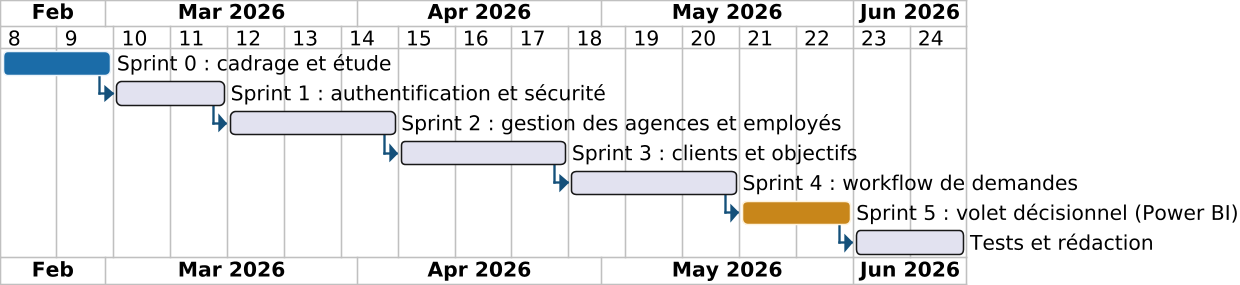
\includegraphics[width=\textwidth]{gantt.png}
  \caption{Planning prévisionnel du projet (diagramme de Gantt)}
  \label{fig:gantt}
\end{figure}

\section*{Conclusion}
Ce chapitre a posé le cadre du projet : l'organisme d'accueil et ses missions,
l'étude de l'existant qui a mis en évidence la problématique, la solution
proposée, ainsi que la démarche et la planification retenues. Le chapitre suivant
est consacré à l'\textbf{analyse et à la spécification des besoins}.
     % Ch.1 — Cadre général du projet
% ===================== CHAPITRE 2 — SPRINT 0 =========================
\chapter{Sprint 0 : Analyse et Spécification des Besoins}

% --- macro locale : logo d'outil non flottant, légendé et numéroté ---
\newcommand{\logofig}[3]{%  #1 = fichier (dossier logos/), #2 = hauteur, #3 = légende
\par\medskip\noindent
\begin{minipage}{\linewidth}\centering
\includegraphics[height=#2]{logos/#1}\par\smallskip
\captionof{figure}{#3}
\end{minipage}\par\medskip}

\section*{Introduction}
Ce chapitre constitue le \emph{Sprint~0}, phase de cadrage qui précède les sprints
de réalisation. Il identifie les acteurs et spécifie les besoins fonctionnels et
non fonctionnels, formalise le pilotage Scrum et le \emph{backlog} produit,
présente les diagrammes de cas d'utilisation global et de classes, planifie les
sprints, puis décrit l'environnement de développement et l'architecture du
système.

% ----------------------------------------------------------------------
\section{Étude du contexte}

\subsection{Identification des acteurs}
Trois profils interagissent avec l'application, conformément aux rôles gérés par
le module de sécurité (table \texttt{SECURITY\_USERS}). Le
tableau~\ref{tab:acteurs} en précise les responsabilités.

\begin{table}[htbp]
\centering
\caption{Identification des acteurs}
\label{tab:acteurs}
\renewcommand{\arraystretch}{1.25}
\begin{tabularx}{\textwidth}{>{\bfseries}p{4cm}X}
\toprule
\textmd{\textbf{Acteur}} & \textbf{Responsabilités}\\
\midrule
Administrateur (\texttt{ADMIN}) & Gère les agences, les employés et les clients ;
valide les demandes de création de clients et d'employés ; consulte le journal
d'audit ; supervise le volet décisionnel.\\
Directeur commercial (\texttt{DIRECTEUR\_COMMERCIAL}) & Soumet les demandes de
création (clients, employés) ; valide les demandes de modification des données
des employés ; consulte les objectifs et les indicateurs.\\
Utilisateur (\texttt{USER}) & Consulte les données autorisées, effectue son
pointage et soumet des demandes de modification de ses propres informations.\\
\bottomrule
\end{tabularx}
\end{table}

\subsection{Spécification des besoins}

\subsubsection{Besoins fonctionnels}
Le système doit permettre :
\begin{itemize}[noitemsep]
  \item l'authentification sécurisée et la gestion des rôles et des droits
        d'accès (\texttt{ADMIN}, \texttt{DIRECTEUR\_COMMERCIAL}, \texttt{USER}) ;
  \item la gestion (CRUD) des agences, des employés et des clients ;
  \item la consultation des objectifs commerciaux et le suivi de la production ;
  \item le \textbf{pointage (présence) des employés} : saisie de l'heure d'arrivée
        et de départ, statut (présent / retard / absent), en mode automatique
        (bouton) ou manuel (administrateur) ;
  \item la soumission et la validation des demandes (clients, employés,
        modifications) selon le cycle \texttt{EN\_ATTENTE} $\rightarrow$
        \texttt{EN\_COURS} $\rightarrow$ \texttt{EFFECTUE}/\texttt{REFUSE} ;
  \item la notification des demandes en attente et la journalisation des actions ;
  \item la consolidation des données par une chaîne \textbf{ETL} et la restitution
        d'indicateurs via un tableau de bord et Power BI ;
  \item la \textbf{segmentation des agences} par apprentissage non supervisé.
\end{itemize}

\subsubsection{Besoins non fonctionnels}
Le tableau~\ref{tab:bnf} récapitule les besoins non fonctionnels.

\begin{table}[htbp]
\centering
\caption{Besoins non fonctionnels}
\label{tab:bnf}
\renewcommand{\arraystretch}{1.2}
\begin{tabularx}{\textwidth}{>{\bfseries}p{3.4cm}X}
\toprule
\textmd{\textbf{Besoin}} & \textbf{Description}\\
\midrule
Sécurité & Authentification, gestion des rôles et protection des opérations
sensibles par des workflows de validation.\\
Fiabilité & Intégrité des données garantie par le SGBD et les transactions JTA.\\
Performance & Temps de réponse acceptable sur les volumes manipulés.\\
Ergonomie & Interface claire et cohérente, navigation par menu latéral.\\
Maintenabilité & Architecture en couches, code modulaire et faiblement couplé.\\
Portabilité & Application Jakarta EE standard, déployable sur serveur compatible.\\
\bottomrule
\end{tabularx}
\end{table}

% ----------------------------------------------------------------------
\section{Pilotage du projet avec Scrum}
Le pilotage du projet repose sur la méthode \textbf{Scrum} présentée au chapitre
précédent. Le tableau~\ref{tab:roles_scrum} précise la répartition des rôles
adoptée durant le stage.

\begin{table}[htbp]
\centering
\caption{Répartition des rôles Scrum du projet}
\label{tab:roles_scrum}
\renewcommand{\arraystretch}{1.2}
\begin{tabularx}{\textwidth}{>{\bfseries}p{3.6cm}p{3.8cm}X}
\toprule
\textmd{\textbf{Rôle}} & \textbf{Assuré par} & \textbf{Mission}\\
\midrule
Product Owner & Maître de stage (BTK) & Exprime et priorise les besoins,
valide les fonctionnalités livrées.\\
Scrum Master & Encadrant académique & Veille au respect de la démarche Scrum et
au bon déroulement des itérations.\\
Équipe de développement & Étudiant & Prend en charge l'analyse, la conception, le
développement et les tests.\\
\bottomrule
\end{tabularx}
\end{table}

% ----------------------------------------------------------------------
\section{Backlog du produit}
Le \emph{product backlog} constitue la liste ordonnée et évolutive des besoins,
exprimés sous forme de \emph{user stories} priorisées selon leur valeur métier.
Il guide la planification des sprints et sert de source unique de travail. Le
tableau~\ref{tab:backlog} en présente le contenu.

\begin{table}[htbp]
\centering
\caption{Backlog produit de l'application}
\label{tab:backlog}
\renewcommand{\arraystretch}{1.2}
\begin{tabularx}{\textwidth}{>{\bfseries}p{0.7cm}p{2.6cm}>{\bfseries}p{1cm}Xp{1.5cm}}
\toprule
\textmd{\textbf{ID}} & \textbf{Fonctionnalité} & \textmd{\textbf{US}} &
\textbf{User story} & \textbf{Priorité}\\
\midrule
01 & Authentification et sécurité & US1 & S'authentifier avec identifiant et mot de passe. & Haute\\
   &                              & US2 & Gérer les rôles et les droits d'accès. & Haute\\
\midrule
02 & Gestion des agences & US3 & Gérer les agences (créer, consulter, modifier, supprimer). & Haute\\
\midrule
03 & Gestion des employés & US4 & Gérer les employés et leur rattachement aux agences. & Haute\\
   &                      & US5 & Gérer les gestionnaires et leurs portefeuilles. & Moyenne\\
\midrule
04 & Gestion des clients & US6 & Gérer les clients (portefeuille). & Moyenne\\
   &                     & US7 & Affecter un client à un gestionnaire. & Moyenne\\
\midrule
05 & Objectifs commerciaux & US8 & Suivre les objectifs commerciaux et la production. & Moyenne\\
\midrule
06 & Pointage & US9 & Pointer la présence (arrivée / départ). & Haute\\
   &          & US10 & Saisir ou corriger un pointage manuel. & Moyenne\\
\midrule
07 & Workflow de demandes & US11 & Soumettre une demande (client, employé, modification). & Moyenne\\
   &                      & US12 & Valider ou refuser une demande. & Moyenne\\
   &                      & US13 & Recevoir des notifications et consulter le journal d'audit. & Moyenne\\
\midrule
08 & Volet décisionnel & US14 & Alimenter le datamart via la chaîne ETL. & Haute\\
   &                   & US15 & Consulter le tableau de bord décisionnel. & Haute\\
   &                   & US16 & Consulter les rapports Power BI. & Moyenne\\
\midrule
09 & Segmentation (IA) & US17 & Segmenter les agences par apprentissage non supervisé. & Moyenne\\
\bottomrule
\end{tabularx}
\end{table}

% ----------------------------------------------------------------------
\section{Diagramme de cas d'utilisation global}
La figure~\ref{fig:uc_global} présente le \textbf{diagramme de cas d'utilisation
global}, qui représente d'un point de vue fonctionnel les interactions entre les
acteurs et les services offerts par le système.

\begin{landscape}
\thispagestyle{plain}
\centering
\vspace*{0.2cm}
\makebox[\linewidth][c]{%
  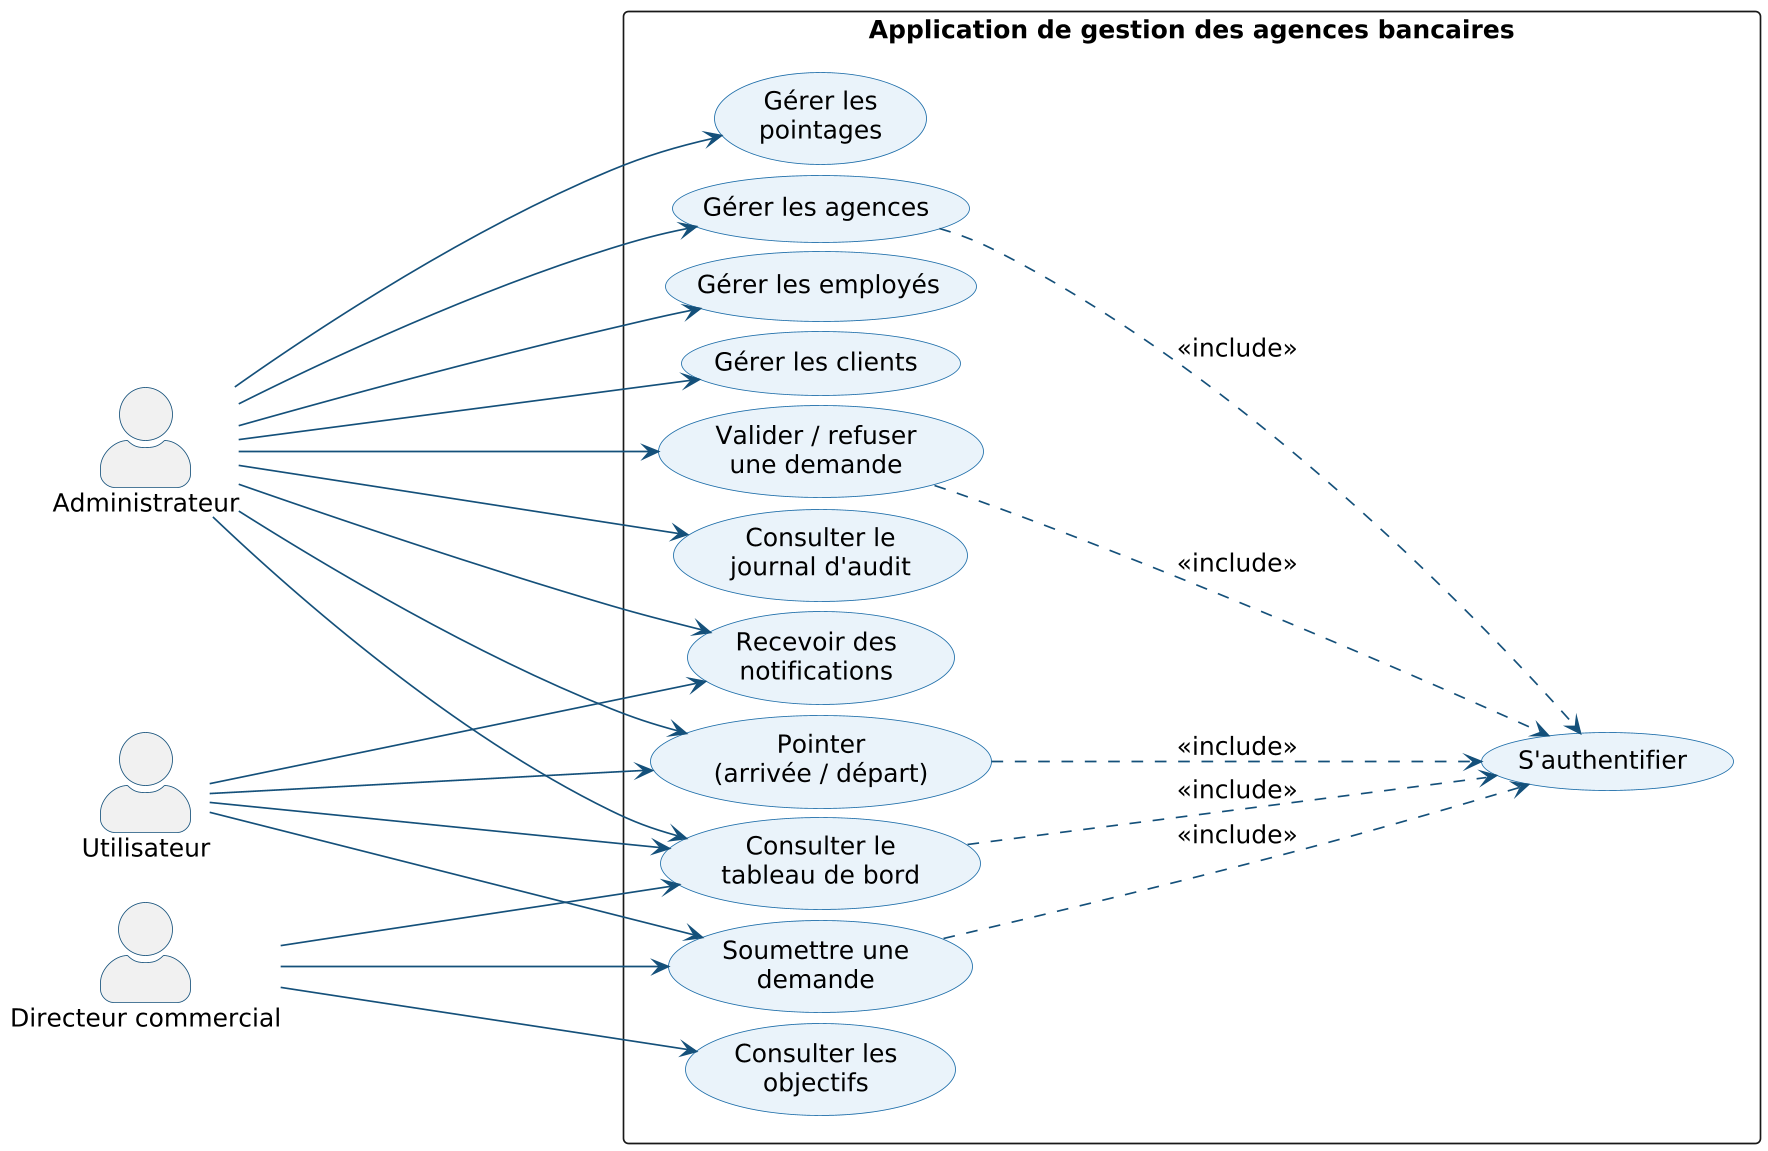
\includegraphics[width=24cm,height=14.2cm,keepaspectratio]{uc_global.png}}
\par\vspace{0.3cm}
\captionof{figure}{Diagramme de cas d'utilisation global}
\label{fig:uc_global}
\end{landscape}

On y distingue les trois acteurs et leurs cas d'utilisation respectifs. Le cas
\emph{S'authentifier} est commun à tous ; il est relié aux autres par une relation
\texttt{\guillemotleft include\guillemotright}, l'accès aux fonctionnalités exigeant une
authentification préalable. L'\textbf{administrateur} concentre les cas de gestion
et de validation ; le \textbf{directeur commercial} soumet les demandes et consulte
les indicateurs ; l'\textbf{utilisateur} se limite à la consultation, au pointage
et aux demandes le concernant.

% ----------------------------------------------------------------------
\section{Diagramme de classe}
La figure~\ref{fig:class} présente le \textbf{diagramme de classes} du modèle
métier, qui représente les entités persistantes du domaine, leurs attributs et
les associations qui les relient.

\begin{figure}[htbp]
  \centering
  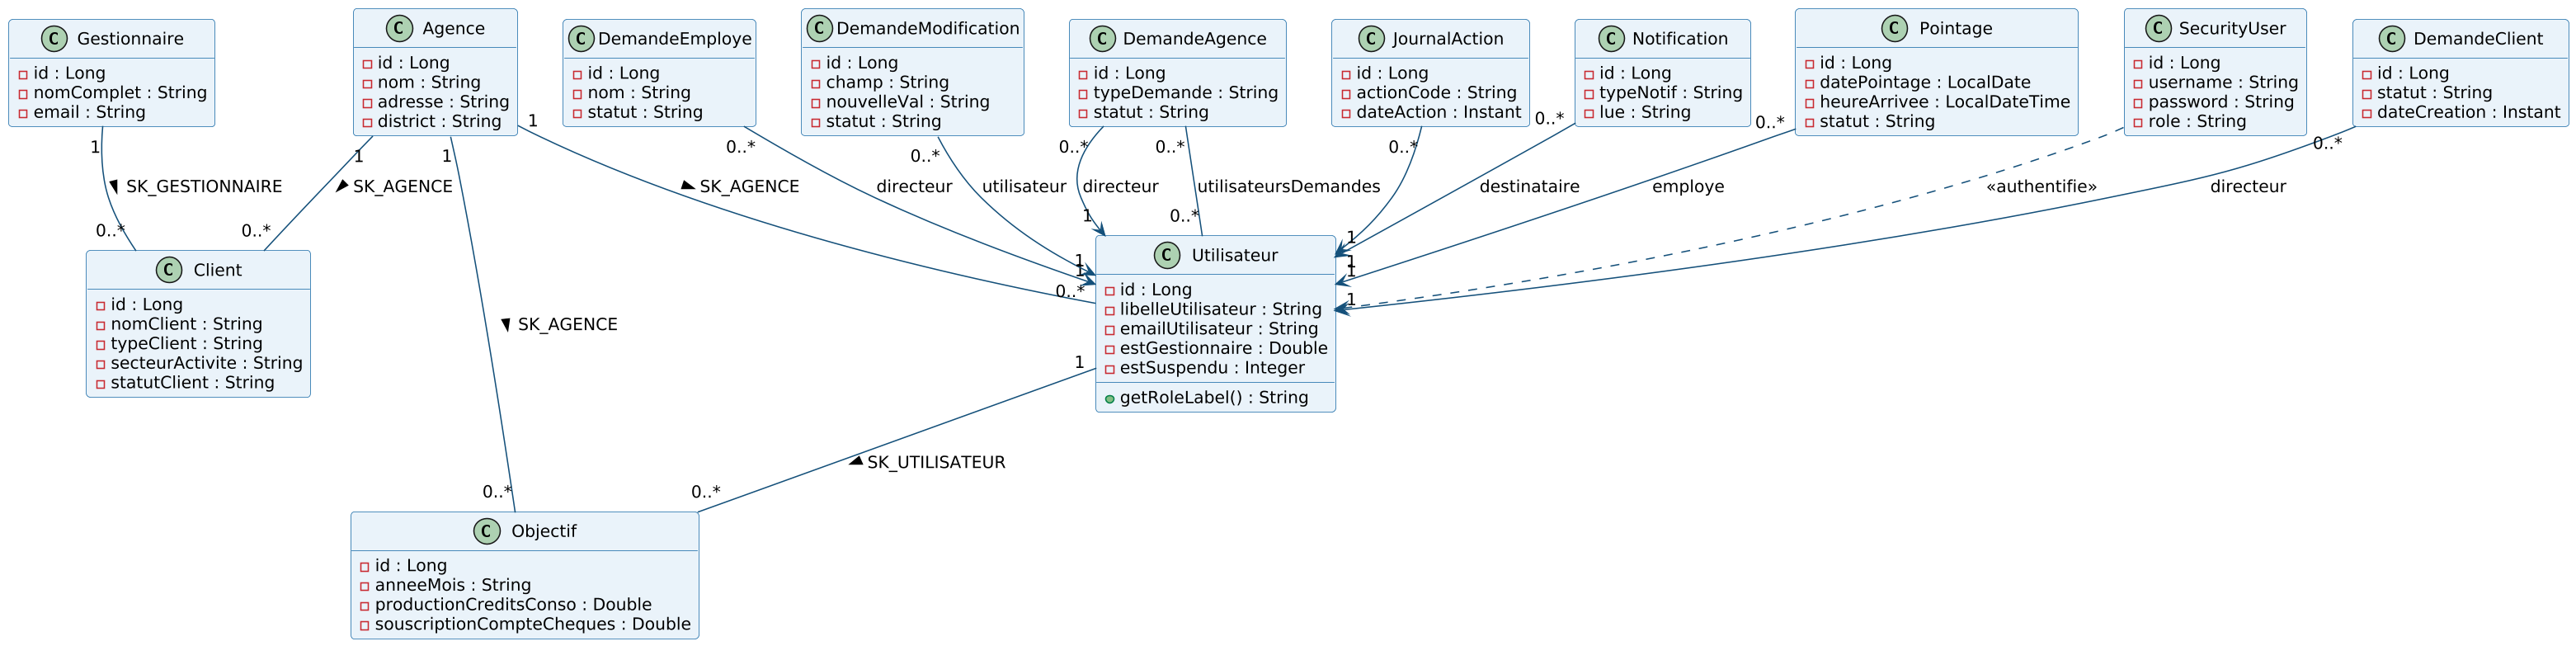
\includegraphics[width=\textwidth]{class.png}
  \caption{Diagramme de classes du modèle métier}
  \label{fig:class}
\end{figure}

L'entité \textbf{\texttt{Utilisateur}} occupe une position centrale. Une
\texttt{Agence} regroupe plusieurs \texttt{Utilisateur}, \texttt{Client} et
\texttt{Objectif} ; un \texttt{Gestionnaire} encadre plusieurs \texttt{Client} ;
les entités de demande (\texttt{DemandeClient}, \texttt{DemandeEmploye},
\texttt{DemandeModification}, \texttt{DemandeAgence}), ainsi que
\texttt{JournalAction}, \texttt{Notification} et \texttt{Pointage}, référencent un
\texttt{Utilisateur} par une association \texttt{@ManyToOne}. Enfin,
\texttt{SecurityUser} est relié à \texttt{Utilisateur} par une dépendance
d'authentification. Le modèle ne comporte ni héritage ni composition : les liens
sont exclusivement des associations, reflétant fidèlement le code du projet.

% ----------------------------------------------------------------------
\section{Planification des sprints}
Conformément au backlog, le développement a été découpé en \textbf{six sprints}
de réalisation, précédés du Sprint~0 de cadrage. Le projet s'est déroulé sur
quatre mois (16 février -- 16 juin 2026). Le tableau~\ref{tab:sprints} détaille
cette planification et la figure~\ref{fig:gantt} en donne le diagramme de Gantt.

\begin{table}[htbp]
\centering
\caption{Planification des sprints}
\label{tab:sprints}
\renewcommand{\arraystretch}{1.2}
\begin{tabularx}{\textwidth}{>{\bfseries}p{1.7cm}p{2cm}p{3.2cm}X}
\toprule
\textmd{\textbf{Sprint}} & \textbf{Durée} & \textbf{User stories} &
\textbf{Objectif du sprint}\\
\midrule
Sprint 1 & 2 semaines & US1, US2 & Authentification et gestion des rôles.\\
Sprint 2 & 2 semaines & US3, US4, US5 & Gestion des agences et des employés.\\
Sprint 3 & 2 semaines & US6, US7, US8 & Gestion des clients et des objectifs.\\
Sprint 4 & 2 semaines & US9--US13 & Pointage, demandes et notifications.\\
Sprint 5 & 3 semaines & US14, US15, US16 & Chaîne ETL et volet décisionnel.\\
Sprint 6 & 2 semaines & US17 & Segmentation des agences (clustering).\\
\bottomrule
\end{tabularx}
\end{table}

\begin{figure}[htbp]
  \centering
  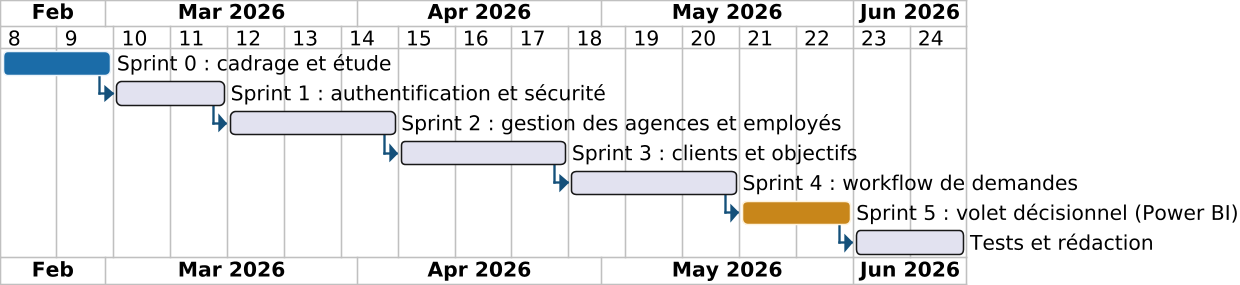
\includegraphics[width=\textwidth]{gantt.png}
  \caption{Planification du projet (diagramme de Gantt des sprints)}
  \label{fig:gantt}
\end{figure}

% ----------------------------------------------------------------------
\section{Environnement de développement}

\subsection{Environnement matériel}
Le développement a été réalisé sur un poste de travail standard : ordinateur
portable doté d'un processeur Intel Core~i5, de 16~Go de mémoire vive et du
système d'exploitation Windows~11.

\subsection{Outil de rédaction du rapport}
Le présent rapport a été rédigé avec \textbf{\LaTeX}, système de composition de
documents particulièrement adapté aux écrits scientifiques et techniques.
\logofig{latex.png}{2.2cm}{Logo de « \LaTeX »}

\subsection{Environnement de développement logiciel}
Plusieurs outils et technologies ont été mobilisés pour la réalisation du projet.

\textbf{Java (JDK~21)} : langage et plateforme d'exécution sur lesquels repose
l'ensemble de l'application.
\logofig{java.png}{2.4cm}{Logo de « Java (JDK 21) »}

\textbf{Jakarta EE~10} : ensemble de spécifications d'entreprise (Servlets, JSP,
EJB, JPA) structurant l'application en couches.
\logofig{jakartaee.png}{2.4cm}{Logo de « Jakarta EE »}

\textbf{Hibernate} : implémentation de JPA assurant le mapping objet-relationnel
entre les entités Java et la base Oracle.
\logofig{hibernate.png}{2.2cm}{Logo de « Hibernate »}

\textbf{Oracle Database} : système de gestion de base de données relationnelle
hébergeant l'ensemble des données opérationnelles et les vues décisionnelles.
\logofig{oracle.png}{1.6cm}{Logo d'« Oracle Database »}

\textbf{WildFly / JBoss} : serveur d'applications Jakarta EE sur lequel
l'application est déployée sous forme d'archive WAR.
\logofig{wildfly.png}{2.2cm}{Logo de « WildFly / JBoss »}

\textbf{Apache Maven} : outil de gestion des dépendances et d'automatisation du
\emph{build} (production du WAR).
\logofig{maven.png}{2cm}{Logo d'« Apache Maven »}

\textbf{IntelliJ IDEA} : environnement de développement intégré utilisé pour le
développement, le débogage et le déploiement de l'application.
\logofig{intellij.png}{2.4cm}{Logo d'« IntelliJ IDEA »}

\textbf{Git et GitHub} : système de gestion de versions et plateforme
d'hébergement du code source.
\par\medskip\noindent
\begin{minipage}{\linewidth}\centering

\includegraphics[height=2.2cm]{logos/git.png}\hspace{1.5cm}%

\includegraphics[height=2.2cm]{logos/github.png}\par\smallskip
\captionof{figure}{Logos de « Git » et « GitHub »}
\end{minipage}\par\medskip

\textbf{ApexCharts} : bibliothèque JavaScript de visualisation utilisée pour les
graphiques du tableau de bord embarqué.
\logofig{apexcharts.png}{2cm}{Logo d'« ApexCharts »}

\textbf{Microsoft Power BI} : outil de \emph{reporting} décisionnel connecté aux
vues analytiques de la base Oracle.
\logofig{powerbi.png}{2.2cm}{Logo de « Microsoft Power BI »}

\textbf{Python} : langage utilisé pour la chaîne \textbf{ETL} et la
\textbf{segmentation} des agences, au moyen des bibliothèques \textbf{pandas}
(manipulation des données) et \textbf{scikit-learn} (apprentissage automatique).
\par\medskip\noindent
\begin{minipage}{\linewidth}\centering

\includegraphics[height=2.2cm]{logos/python.png}\hspace{1.2cm}%

\includegraphics[height=2.2cm]{logos/pandas.png}\hspace{1.2cm}%

\includegraphics[height=2.2cm]{logos/scikitlearn.png}\par\smallskip
\captionof{figure}{Logos de « Python », « pandas » et « scikit-learn »}
\end{minipage}\par\medskip

% ----------------------------------------------------------------------
\section{Architecture du système}
L'architecture définit l'organisation des composants du système et la manière dont
ils communiquent. Elle est présentée à trois niveaux : globale, physique et
logique.

\subsection{Architecture globale}
L'architecture globale (figure~\ref{fig:archi_globale}) offre une vue d'ensemble
des composants. Un poste client (navigateur) dialogue en \texttt{HTTP/HTTPS} avec
l'application web déployée sur \textbf{WildFly}, structurée en couches
(présentation, contrôle, métier, persistance) ; celle-ci accède à la base
\textbf{Oracle} en JDBC. La base alimente, d'une part, \textbf{Power BI} via les
vues \texttt{V\_BI\_*} et, d'autre part, la \textbf{chaîne décisionnelle Python}
(ETL puis segmentation).

\begin{figure}[htbp]
  \centering
  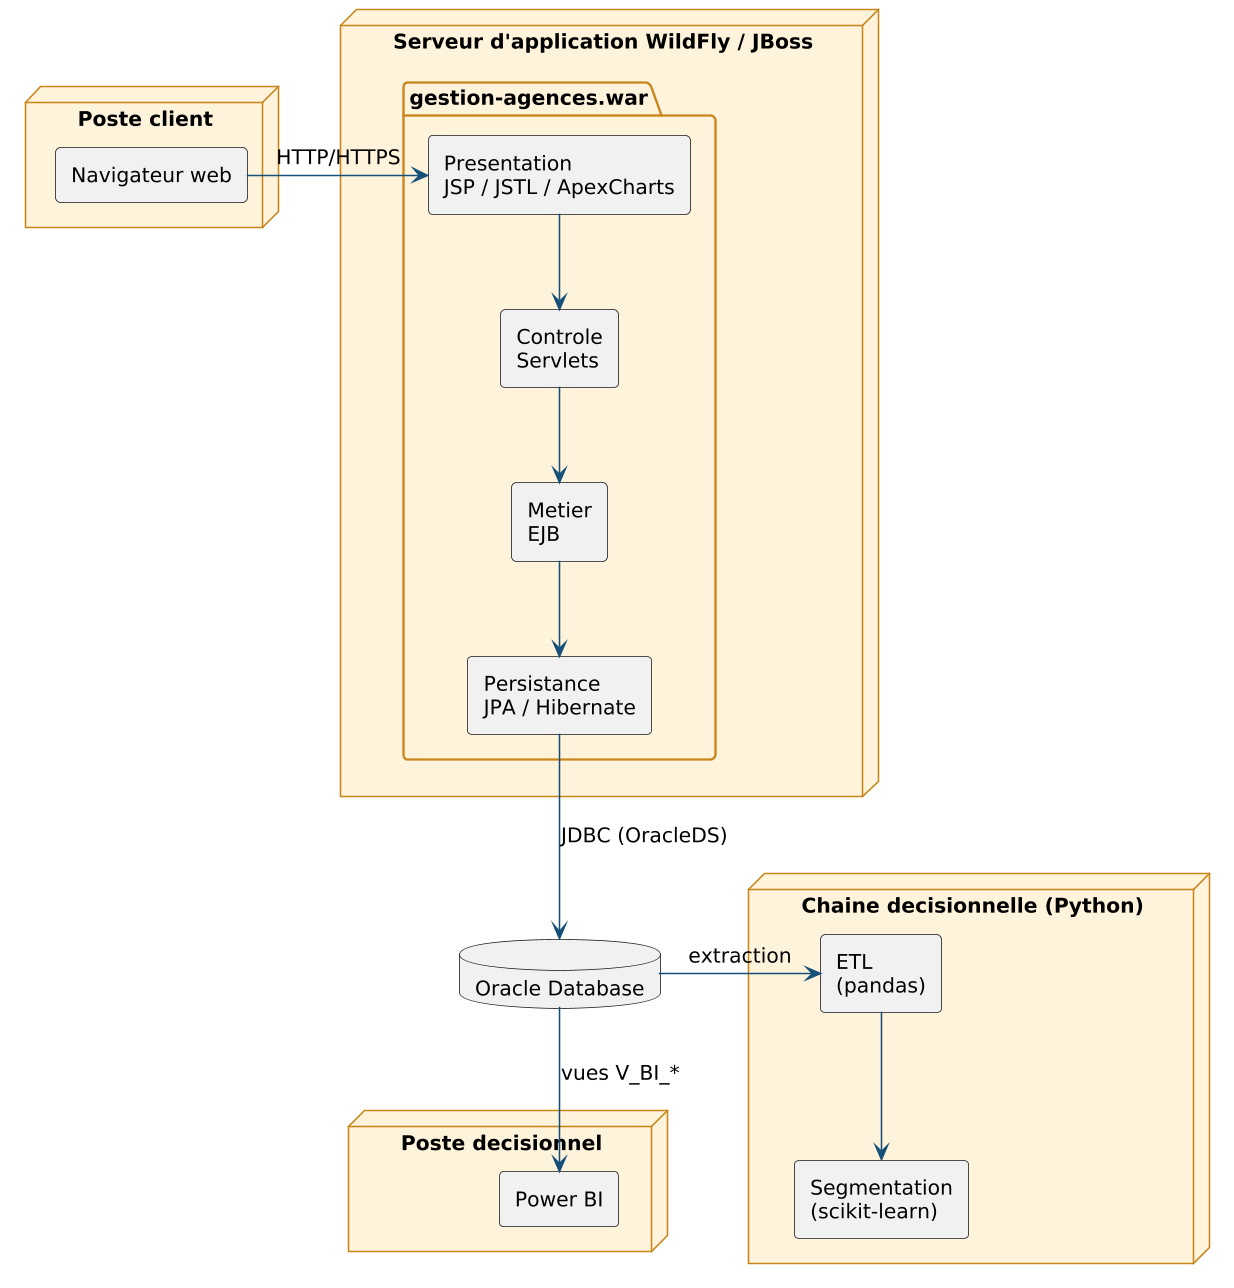
\includegraphics[width=0.92\textwidth]{archi_globale.png}
  \caption{Architecture globale du système}
  \label{fig:archi_globale}
\end{figure}

\subsection{Architecture physique}
L'architecture physique (figure~\ref{fig:archi_physique}) représente le
\textbf{déploiement} des composants sur les nœuds matériels selon une organisation
\textbf{3-tiers} : le poste client, le serveur d'applications WildFly hébergeant
\texttt{gestion-agences.war} (accès à la base via la source de données JTA
\texttt{OracleDS}), le serveur de base de données Oracle (\texttt{FREEPDB1}) et le
poste décisionnel exécutant Power BI.

\begin{figure}[htbp]
  \centering
  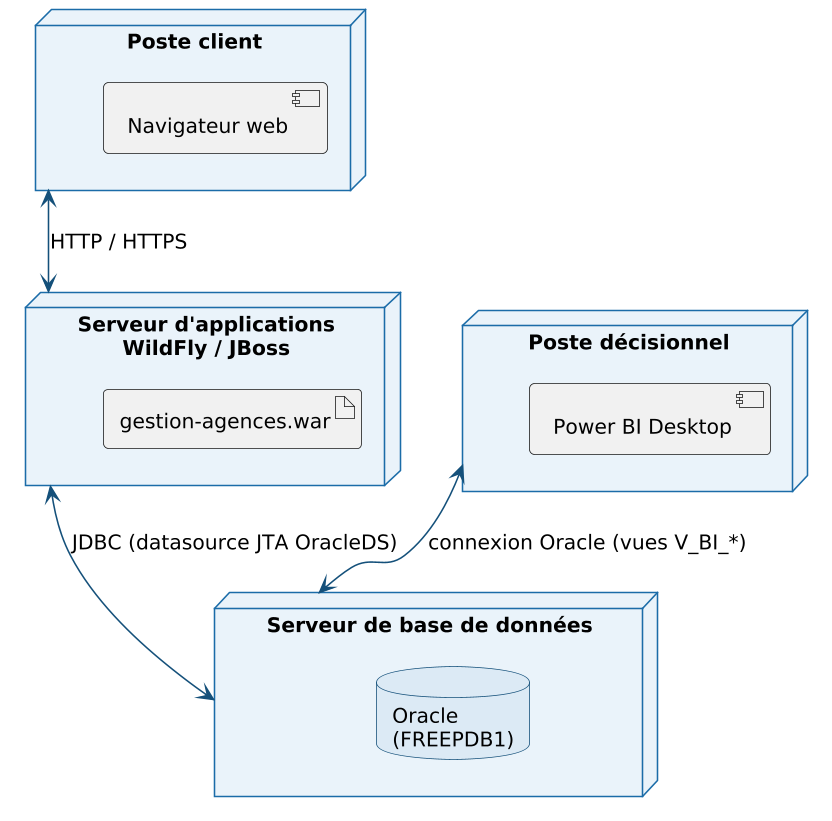
\includegraphics[width=0.85\textwidth]{archi_physique.png}
  \caption{Architecture physique (diagramme de déploiement 3-tiers)}
  \label{fig:archi_physique}
\end{figure}

\subsection{Architecture logique}
L'architecture logique (figure~\ref{fig:archi_logique}) décompose le système en
\textbf{couches} faiblement couplées suivant le patron \textbf{MVC} : la couche
\emph{présentation} (JSP/JSTL, ApexCharts), la couche \emph{contrôle} (Servlets et
le filtre \texttt{NotificationFilter}), la couche \emph{métier} (services EJB) et
la couche \emph{persistance} (entités JPA et Hibernate dialoguant avec Oracle via
l'\texttt{EntityManager}).

\begin{figure}[htbp]
  \centering
  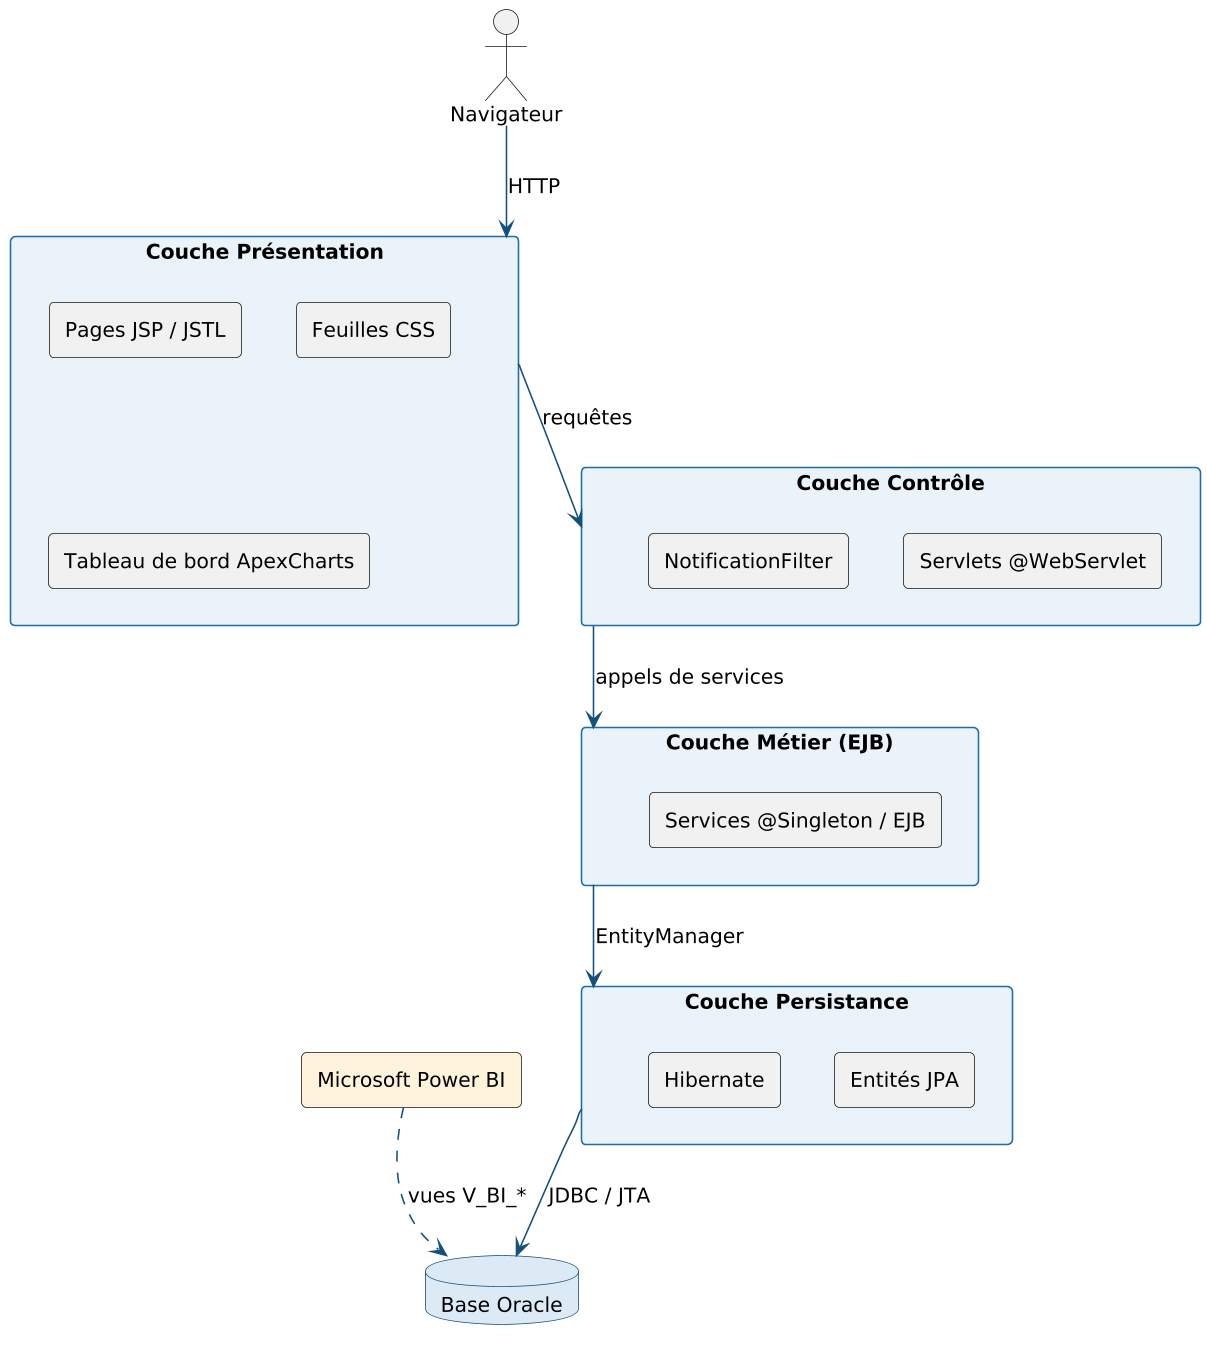
\includegraphics[width=0.62\textwidth]{archi_logique.png}
  \caption{Architecture logique en couches de l'application}
  \label{fig:archi_logique}
\end{figure}

\section*{Conclusion}
Ce Sprint~0 a posé les fondations du projet : acteurs, besoins, backlog priorisé,
planification des sprints, environnement de développement et architecture du
système. Les chapitres suivants détaillent chaque sprint de réalisation, en
commençant par l'authentification et la gestion des rôles.
   % Ch.2 — Sprint 0 : Analyse et spécification
% ===================== CHAPITRE 3 — SPRINT 1 =========================
\chapter{Sprint 1 : Authentification et gestion des rôles}

\section*{Introduction}
Ce chapitre couvre le premier sprint de réalisation, consacré à la sécurité
d'accès. Après un rappel des objectifs, il présente le diagramme de cas
d'utilisation et le \emph{sprint backlog}, l'analyse des besoins, la conception
au moyen d'un diagramme de séquence, puis les interfaces réalisées.

\section{Objectifs du Sprint}
L'objectif de ce sprint est de mettre en place l'\textbf{authentification} des
utilisateurs et la \textbf{gestion des rôles et des droits d'accès}
(\texttt{ADMIN}, \texttt{DIRECTEUR\_COMMERCIAL}, \texttt{USER}), socle de sécurité
de toute l'application.

\section{Spécification des besoins}

\subsection{Diagramme de cas d'utilisation du Sprint 1}
La figure~\ref{fig:uc_s1} présente les cas d'utilisation du sprint.

\begin{figure}[htbp]
  \centering
  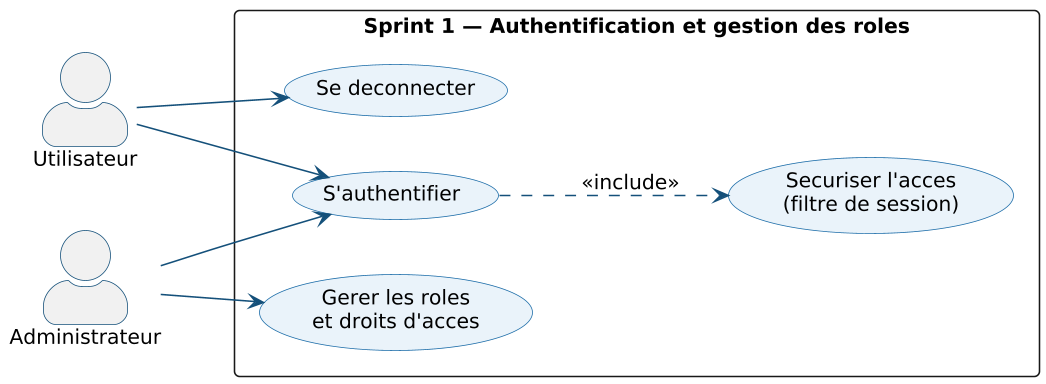
\includegraphics[width=0.82\textwidth]{uc_sprint1.png}
  \caption{Diagramme de cas d'utilisation du Sprint 1}
  \label{fig:uc_s1}
\end{figure}

\subsection{Sprint Backlog du sprint 1}
Le tableau~\ref{tab:bl_s1} détaille les user stories du sprint et les tâches
techniques associées.

\begin{table}[htbp]
\centering
\caption{Sprint Backlog du sprint 1}
\label{tab:bl_s1}
\renewcommand{\arraystretch}{1.3}
\begin{tabularx}{\textwidth}{>{\bfseries}p{1cm}p{5.2cm}X}
\toprule
\textmd{\textbf{US}} & \textbf{User story} & \textbf{Tâches techniques}\\
\midrule
US1 & S'authentifier avec identifiant et mot de passe. &
Créer le \texttt{LoginServlet} (\texttt{POST /login}) ; vérifier les identifiants
via le \texttt{SecurityService} sur la table \texttt{SECURITY\_USERS} ; ouvrir une
\texttt{HttpSession} ; créer le \texttt{LogoutServlet}.\\
\midrule
US2 & Gérer les rôles et les droits d'accès. &
Associer un rôle (\texttt{ADMIN}, \texttt{DIRECTEUR\_COMMERCIAL}, \texttt{USER}) à
chaque utilisateur ; restreindre l'accès aux fonctionnalités selon le rôle ;
gérer la réinitialisation du mot de passe (\texttt{ForgotPasswordServlet}).\\
\bottomrule
\end{tabularx}
\end{table}

\section{Analyse des besoins}

\subsection{Description textuelle des cas d'utilisation}
Les tableaux~\ref{tab:cu_auth} et~\ref{tab:cu_roles} décrivent les cas
d'utilisation principaux du sprint.

\cudesc{tab:cu_auth}{S'authentifier}
{Permettre à l'utilisateur de se connecter à l'application avec son identifiant et
son mot de passe.}
{Administrateur / Directeur commercial / Utilisateur}
{L'utilisateur doit disposer d'un compte actif dans la table \texttt{SECURITY\_USERS}.}
{Une session est ouverte et l'utilisateur est redirigé vers le tableau de bord
correspondant à son rôle.}
{(1) L'utilisateur saisit son identifiant et son mot de passe ; (2) le
\texttt{SecurityService} vérifie les informations sur la table de sécurité ; (3) en
cas de succès, une session est ouverte et l'utilisateur est redirigé ; (4) sinon,
un message d'erreur est affiché.}

\cudesc{tab:cu_roles}{Gérer les rôles et les droits d'accès}
{Permettre à l'administrateur d'attribuer un rôle à chaque utilisateur afin de
contrôler l'accès aux fonctionnalités.}
{Administrateur}
{L'administrateur doit être authentifié avec le rôle \texttt{ADMIN}.}
{Le rôle est enregistré et les droits d'accès de l'utilisateur sont mis à jour.}
{(1) L'administrateur consulte la liste des utilisateurs ; (2) il sélectionne un
utilisateur ; (3) il lui attribue un rôle (\texttt{ADMIN},
\texttt{DIRECTEUR\_COMMERCIAL} ou \texttt{USER}) ; (4) le système applique le
contrôle d'accès correspondant.}

\section{Conception}

\subsection{Diagramme de séquence : « S'authentifier »}
La figure~\ref{fig:seq_auth} décrit le déroulement dynamique de l'authentification.

\begin{figure}[htbp]
  \centering
  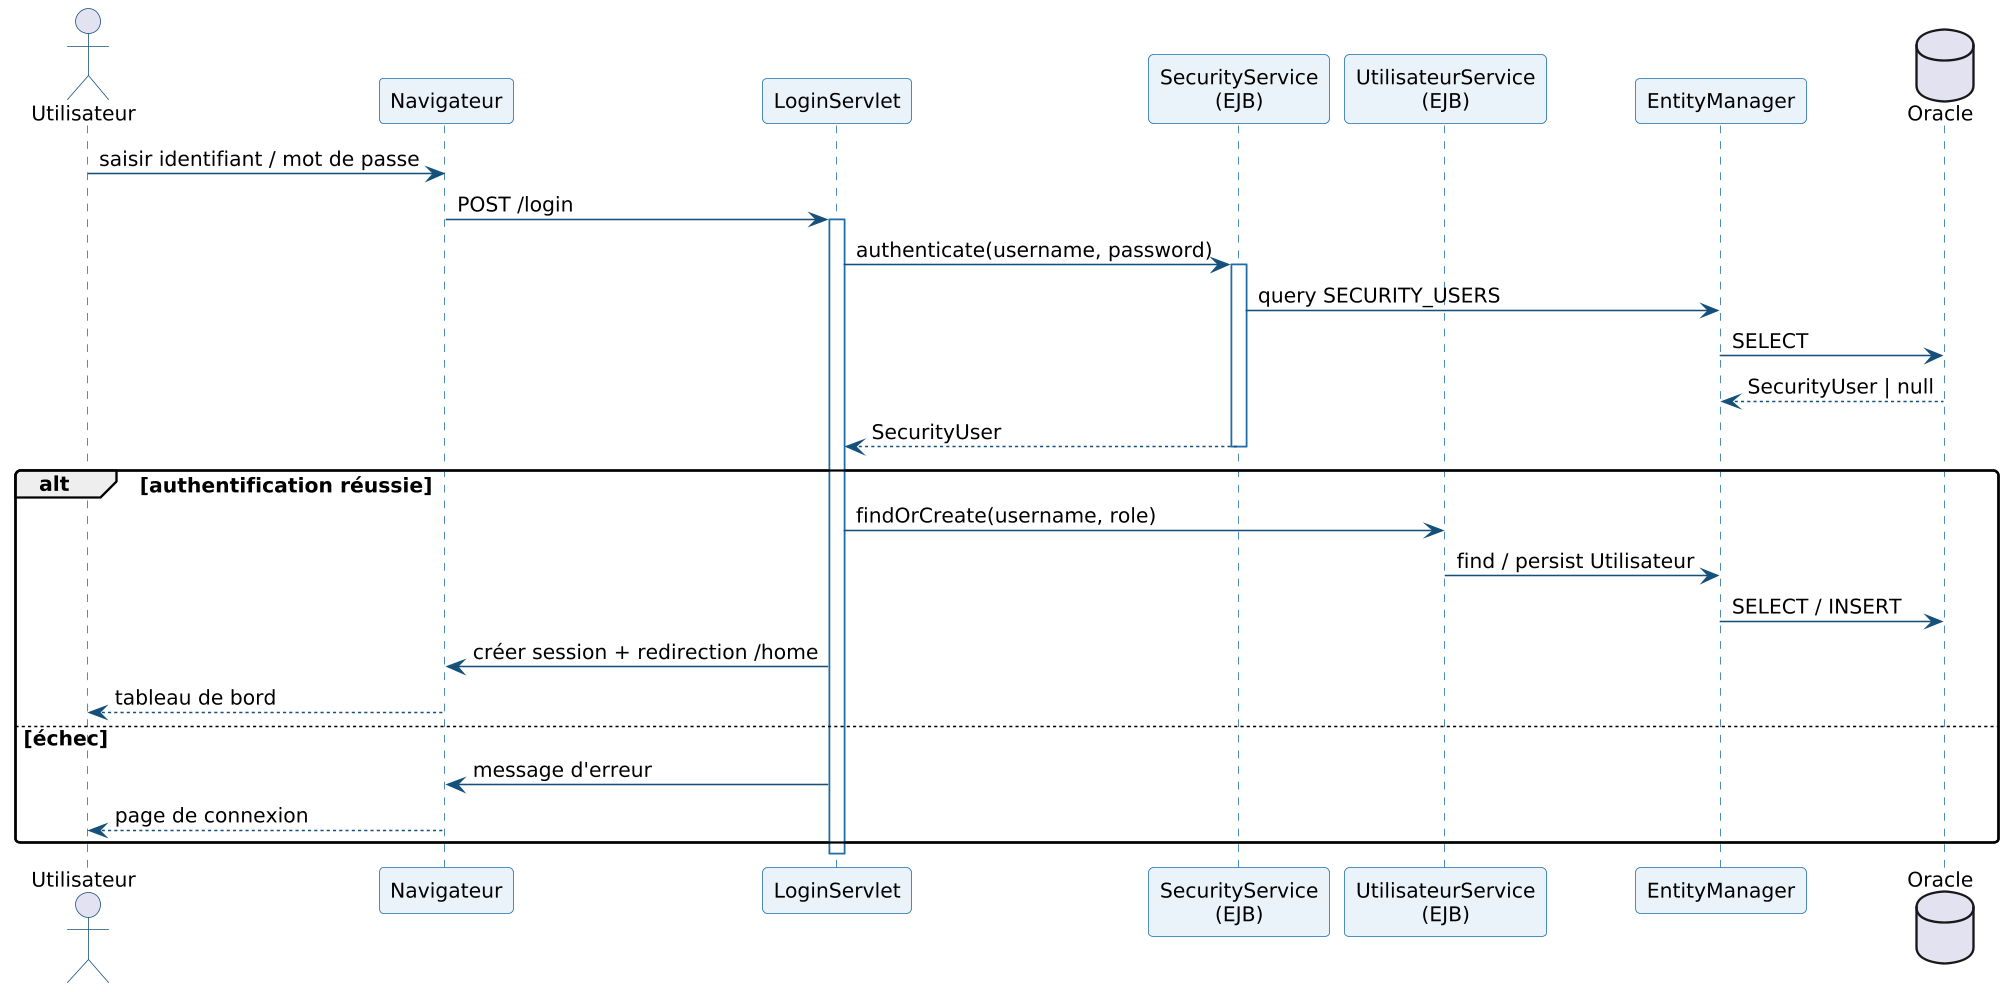
\includegraphics[width=0.92\textwidth]{seq_auth.png}
  \caption{Diagramme de séquence -- Authentification}
  \label{fig:seq_auth}
\end{figure}

Le \texttt{LoginServlet} reçoit la requête \texttt{POST /login} et délègue la
vérification au \texttt{SecurityService}, qui interroge la table
\texttt{SECURITY\_USERS} via l'\texttt{EntityManager}. Le fragment combiné
\texttt{alt} distingue les deux issues : en cas de succès, l'\texttt{Utilisateur}
métier est associé (ou créé), une session est ouverte et l'utilisateur est
redirigé vers le tableau de bord ; en cas d'échec, un message d'erreur est
renvoyé.

\section{Réalisation : interfaces utilisateur}
La figure~\ref{fig:ui_login} présente la page d'authentification réalisée :
l'utilisateur y saisit son identifiant et son mot de passe pour accéder à
l'application.

\begin{figure}[htbp]
  \centering
  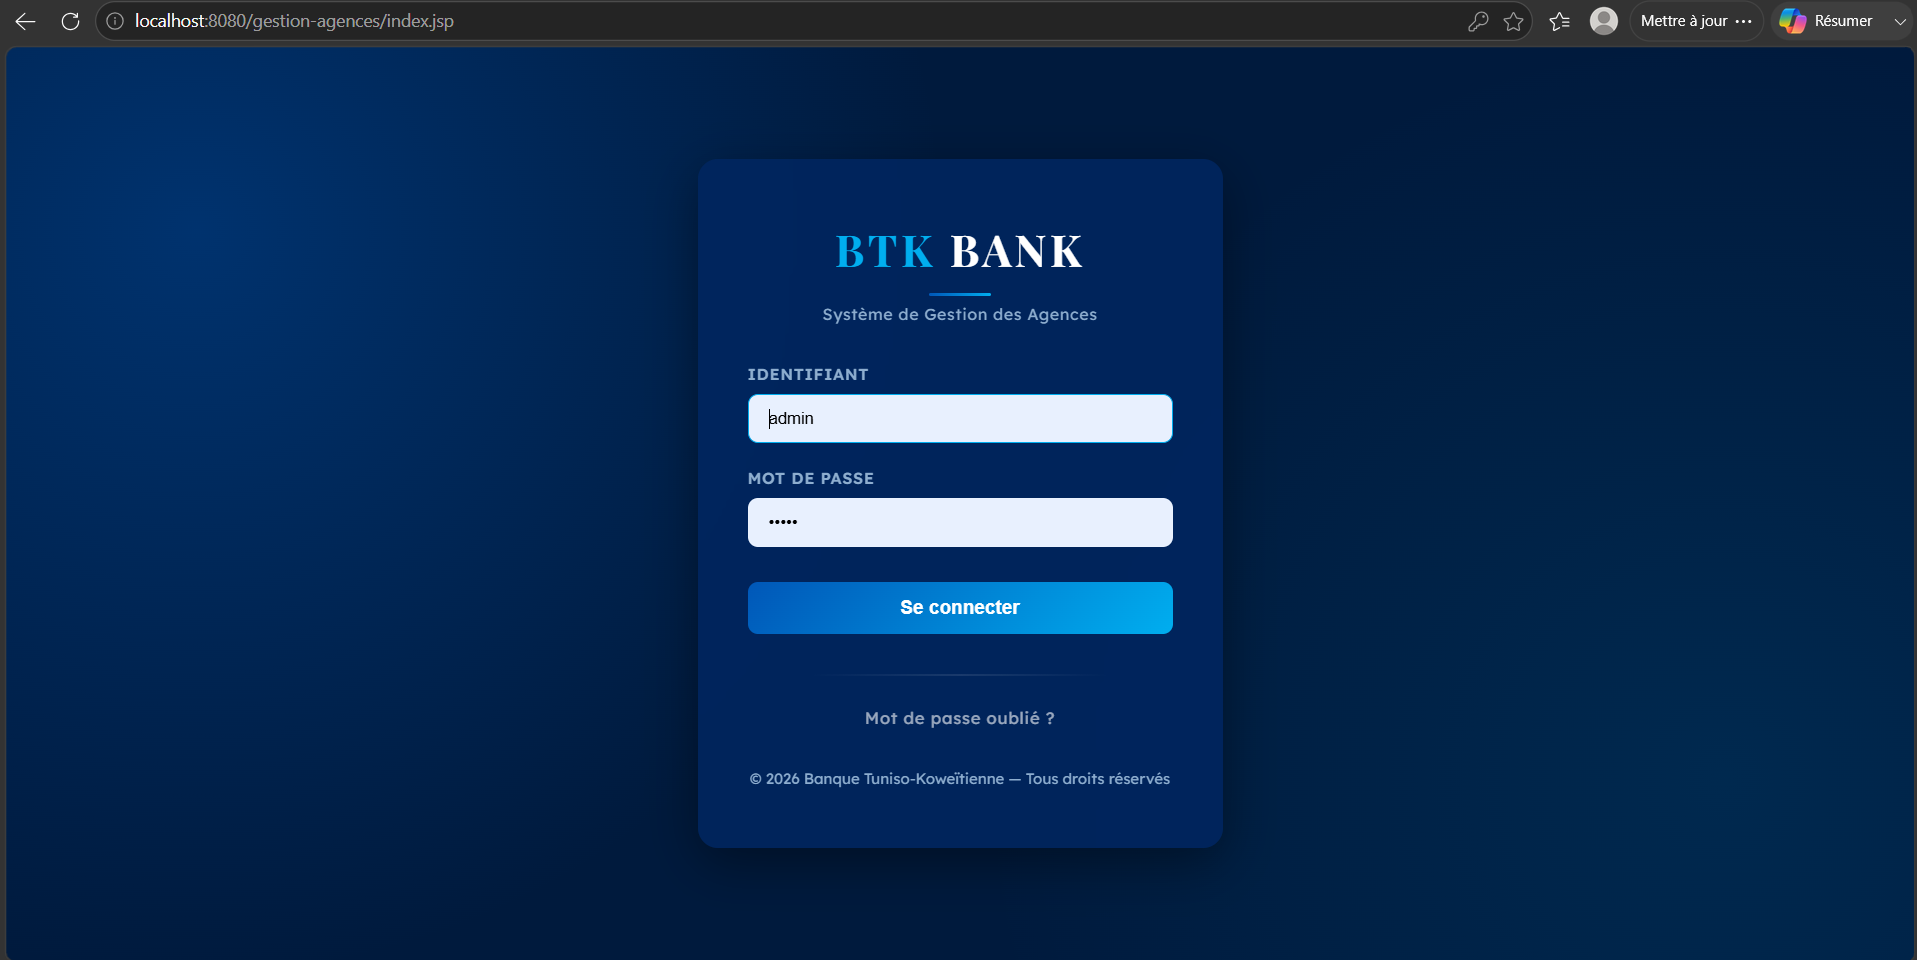
\includegraphics[width=\textwidth]{screens/login.png}
  \caption{Interface d'authentification}
  \label{fig:ui_login}
\end{figure}

\section*{Conclusion}
Ce sprint a mis en place le socle de sécurité de l'application :
l'authentification et la gestion des rôles. Le sprint suivant aborde la gestion
des agences et des employés.
             % Ch.3 — Sprint 1 : Authentification
% ===================== CHAPITRE 4 — SPRINT 2 =========================
\chapter{Sprint 2 : Gestion des agences et des employés}

\section*{Introduction}
Ce sprint met en place les fonctionnalités de gestion du référentiel : les
agences, les employés et leur rattachement. Il suit la même démarche : objectifs,
spécification (cas d'utilisation et backlog), analyse, conception et réalisation.

\section{Objectifs du Sprint}
L'objectif est d'offrir la \textbf{gestion complète (CRUD)} des agences et des
employés, ainsi que le \textbf{rattachement} de chaque employé à son agence et la
gestion des gestionnaires.

\section{Spécification des besoins}

\subsection{Diagramme de cas d'utilisation du Sprint 2}
La figure~\ref{fig:uc_s2} présente les cas d'utilisation du sprint.

\begin{figure}[htbp]
  \centering
  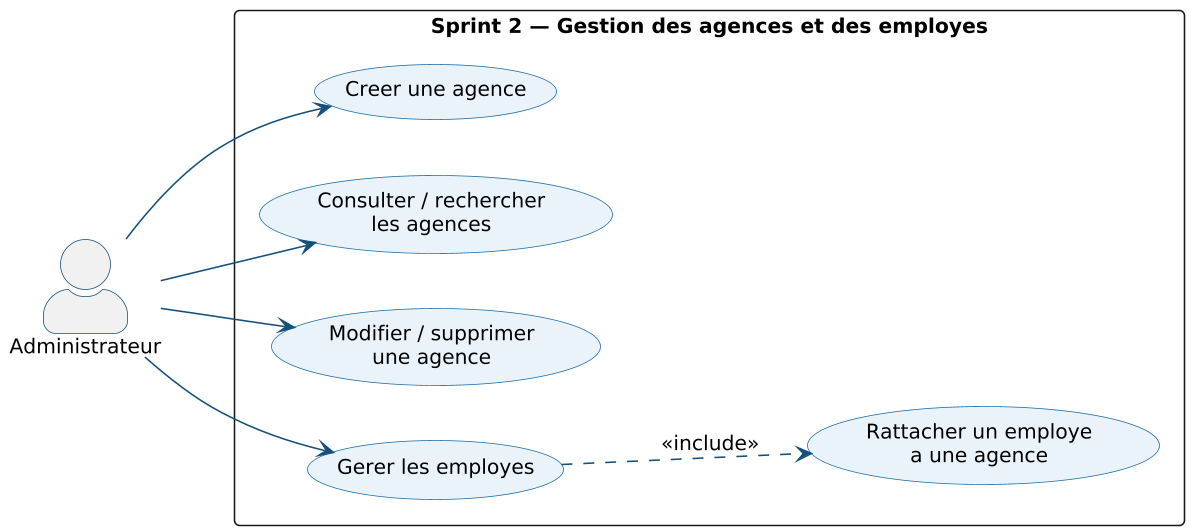
\includegraphics[width=0.82\textwidth]{uc_sprint2.png}
  \caption{Diagramme de cas d'utilisation du Sprint 2}
  \label{fig:uc_s2}
\end{figure}

\subsection{Sprint Backlog du sprint 2}
Le tableau~\ref{tab:bl_s2} détaille les user stories et les tâches techniques.

\begin{table}[htbp]
\centering
\caption{Sprint Backlog du sprint 2}
\label{tab:bl_s2}
\renewcommand{\arraystretch}{1.3}
\begin{tabularx}{\textwidth}{>{\bfseries}p{1cm}p{5.2cm}X}
\toprule
\textmd{\textbf{US}} & \textbf{User story} & \textbf{Tâches techniques}\\
\midrule
US3 & Gérer les agences (créer, consulter, modifier, supprimer). &
Développer l'\texttt{AgenceServlet} et l'\texttt{AgenceService} (EJB) sur l'entité
\texttt{Agence} ; réaliser la page \texttt{agences.jsp} avec les actions CRUD.\\
\midrule
US4 & Gérer les employés et leur rattachement aux agences. &
Développer l'\texttt{AjouterEmployeServlet} et le \texttt{BUtilisateurServlet} ;
gérer les employés via l'\texttt{UtilisateurService} ; associer chaque employé à
une \texttt{Agence} (\texttt{SK\_AGENCE}) ; pages \texttt{employes.jsp} et
\texttt{add-effectif.jsp}.\\
\midrule
US5 & Gérer les gestionnaires et leurs portefeuilles. &
Développer le \texttt{GestionnaireServlet} et le \texttt{GestionnaireService} sur
l'entité \texttt{Gestionnaire} ; page \texttt{gestionnaire.jsp}.\\
\bottomrule
\end{tabularx}
\end{table}

\section{Analyse des besoins}

\subsection{Description textuelle des cas d'utilisation}

\cudesc{tab:cu_agence}{Gérer les agences}
{Permettre à l'administrateur de créer, consulter, modifier et supprimer les
agences du réseau.}
{Administrateur}
{L'administrateur doit être authentifié avec le rôle \texttt{ADMIN}.}
{L'agence créée ou modifiée est enregistrée dans la base et la liste est mise à
jour.}
{(1) L'administrateur accède à l'interface de gestion des agences ; (2) il
sélectionne une action (créer, modifier, supprimer) ; (3) il saisit ou met à jour
les informations de l'agence ; (4) l'\texttt{AgenceService} persiste la
modification et la liste est rafraîchie.}

\cudesc{tab:cu_employe}{Gérer les employés}
{Permettre à l'administrateur de gérer les employés et de les rattacher à leur
agence.}
{Administrateur}
{L'administrateur doit être authentifié et l'agence de rattachement doit exister.}
{L'employé est enregistré et rattaché à son agence.}
{(1) L'administrateur accède à l'interface de gestion des employés ; (2) il saisit
les informations de l'employé ; (3) il sélectionne l'agence de rattachement ; (4)
l'\texttt{UtilisateurService} enregistre l'employé associé à l'agence.}

\section{Conception}

\subsection{Diagramme de séquence : « Créer une agence »}
La figure~\ref{fig:seq_agence} décrit le scénario de création d'une agence.

\begin{figure}[htbp]
  \centering
  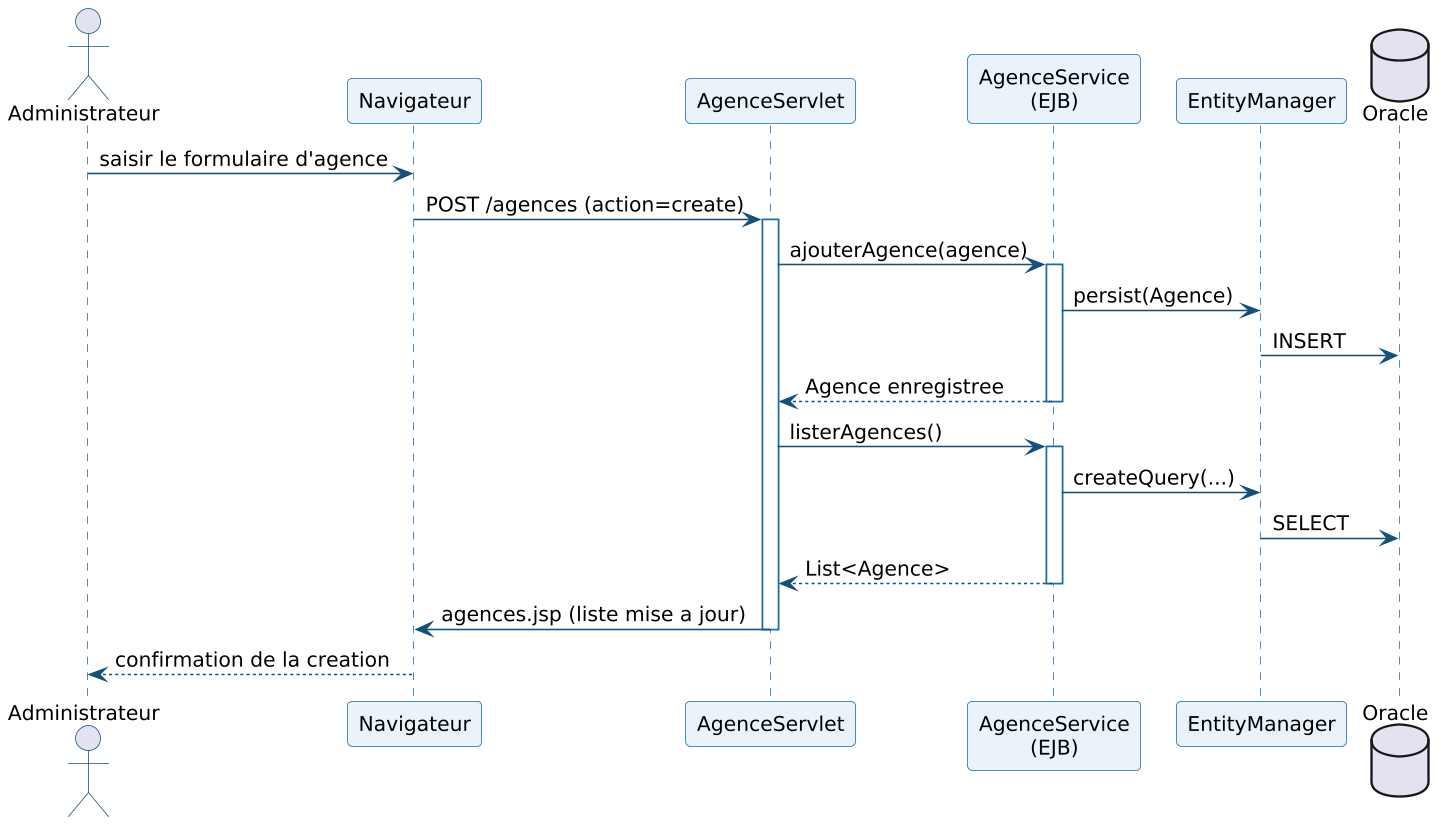
\includegraphics[width=0.92\textwidth]{seq_agence.png}
  \caption{Diagramme de séquence -- Création d'une agence}
  \label{fig:seq_agence}
\end{figure}

L'\texttt{AgenceServlet} reçoit la requête de création et délègue à
l'\texttt{AgenceService}, qui persiste la nouvelle \texttt{Agence} via
l'\texttt{EntityManager} (\texttt{INSERT}), puis recharge la liste des agences
renvoyée à la page \texttt{agences.jsp}. Le même schéma s'applique aux opérations
de modification et de suppression.

\section{Réalisation : interfaces utilisateur}
La figure~\ref{fig:ui_agences} illustre les interfaces de gestion des agences et
des employés. \emph{Les captures d'écran réelles seront insérées à cet emplacement.}

\begin{figure}[htbp]
  \centering
  \fbox{\parbox[c][3.6cm][c]{0.8\textwidth}{\centering\itshape Capture à insérer
  -- gestion des agences et des employés}}
  \caption{Interfaces de gestion des agences et des employés}
  \label{fig:ui_agences}
\end{figure}

\section*{Conclusion}
Ce sprint a doté l'application de la gestion du référentiel des agences et des
employés. Le sprint suivant traite des clients et des objectifs commerciaux.
             % Ch.4 — Sprint 2 : Agences et employés
% ===================== CHAPITRE 5 — SPRINT 3 =========================
\chapter{Sprint 3 : Gestion des clients et des objectifs}

\section*{Introduction}
Ce sprint complète le référentiel commercial : la gestion du portefeuille clients,
leur affectation aux gestionnaires et le suivi des objectifs commerciaux.

\section{Objectifs du Sprint}
L'objectif est de permettre la \textbf{gestion des clients} (portefeuille), leur
\textbf{affectation à un gestionnaire} et le \textbf{suivi des objectifs
commerciaux} (ouvertures de comptes, crédits, épargne) par agence.

\section{Spécification des besoins}

\subsection{Diagramme de cas d'utilisation du Sprint 3}
La figure~\ref{fig:uc_s3} présente les cas d'utilisation du sprint.

\begin{figure}[htbp]
  \centering
  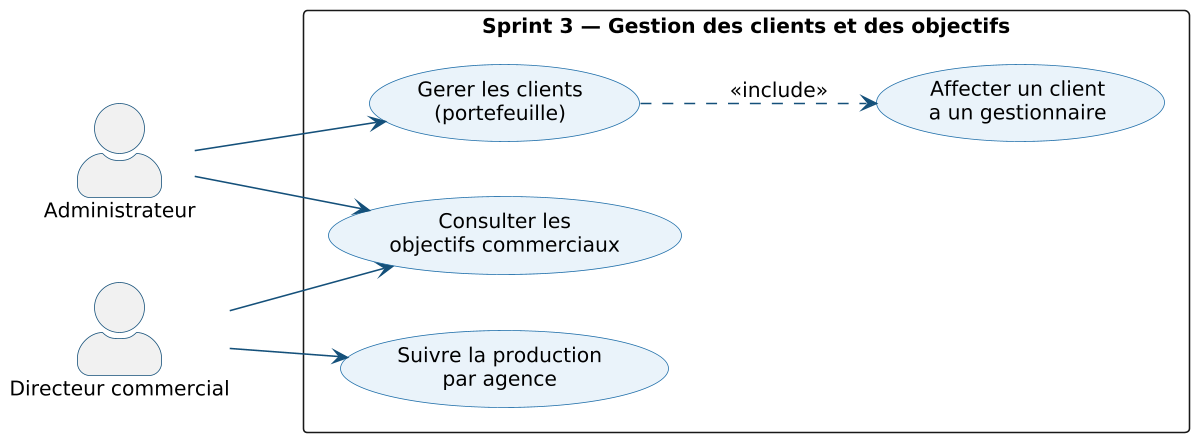
\includegraphics[width=0.82\textwidth]{uc_sprint3.png}
  \caption{Diagramme de cas d'utilisation du Sprint 3}
  \label{fig:uc_s3}
\end{figure}

\subsection{Sprint Backlog du sprint 3}
Le tableau~\ref{tab:bl_s3} détaille les user stories et les tâches techniques.

\begin{table}[htbp]
\centering
\caption{Sprint Backlog du sprint 3}
\label{tab:bl_s3}
\renewcommand{\arraystretch}{1.3}
\begin{tabularx}{\textwidth}{>{\bfseries}p{1cm}p{5.2cm}X}
\toprule
\textmd{\textbf{US}} & \textbf{User story} & \textbf{Tâches techniques}\\
\midrule
US6 & Gérer les clients (portefeuille). &
Développer le \texttt{ClientServlet} et le \texttt{ClientService} sur l'entité
\texttt{Client} ; page \texttt{client.jsp} ; gérer les clients BTK
(\texttt{BClientServlet}, \texttt{clients-btk.jsp}).\\
\midrule
US7 & Affecter un client à un gestionnaire. &
Associer chaque \texttt{Client} à un \texttt{Gestionnaire}
(\texttt{SK\_GESTIONNAIRE}) ; mettre à jour le portefeuille du gestionnaire.\\
\midrule
US8 & Suivre les objectifs commerciaux et la production. &
Développer l'\texttt{ObjectifServlet} et l'\texttt{ObjectifService} sur l'entité
\texttt{Objectif} ; pages \texttt{objectifs.jsp} et \texttt{objectifs-btk.jsp} ;
restituer comptes, crédits et épargne par agence.\\
\bottomrule
\end{tabularx}
\end{table}

\section{Analyse des besoins}

\subsection{Description textuelle des cas d'utilisation}

\cudesc{tab:cu_client}{Gérer les clients}
{Permettre à l'administrateur de gérer le portefeuille clients et d'affecter
chaque client à un gestionnaire.}
{Administrateur}
{L'administrateur doit être authentifié et le gestionnaire de rattachement doit
exister.}
{Le client est enregistré et associé à son gestionnaire dans la base.}
{(1) L'administrateur accède à l'interface de gestion des clients ; (2) il saisit
ou met à jour les informations du client ; (3) il sélectionne le gestionnaire
responsable ; (4) le \texttt{ClientService} enregistre le client et met à jour le
portefeuille.}

\cudesc{tab:cu_objectif}{Suivre les objectifs commerciaux}
{Permettre au directeur commercial de consulter les objectifs et la production par
agence.}
{Directeur commercial / Administrateur}
{L'acteur doit être authentifié et des objectifs doivent être renseignés pour la
période.}
{Les indicateurs de production (comptes, crédits, épargne) sont restitués par
agence.}
{(1) L'acteur accède à l'interface des objectifs ; (2) il sélectionne une agence
et une période ; (3) l'\texttt{ObjectifService} agrège la production ; (4) les
indicateurs sont affichés.}

\section{Conception}

\subsection{Diagramme de séquence : « Gérer un client »}
La figure~\ref{fig:seq_client} décrit l'enregistrement et l'affectation d'un
client.

\begin{figure}[htbp]
  \centering
  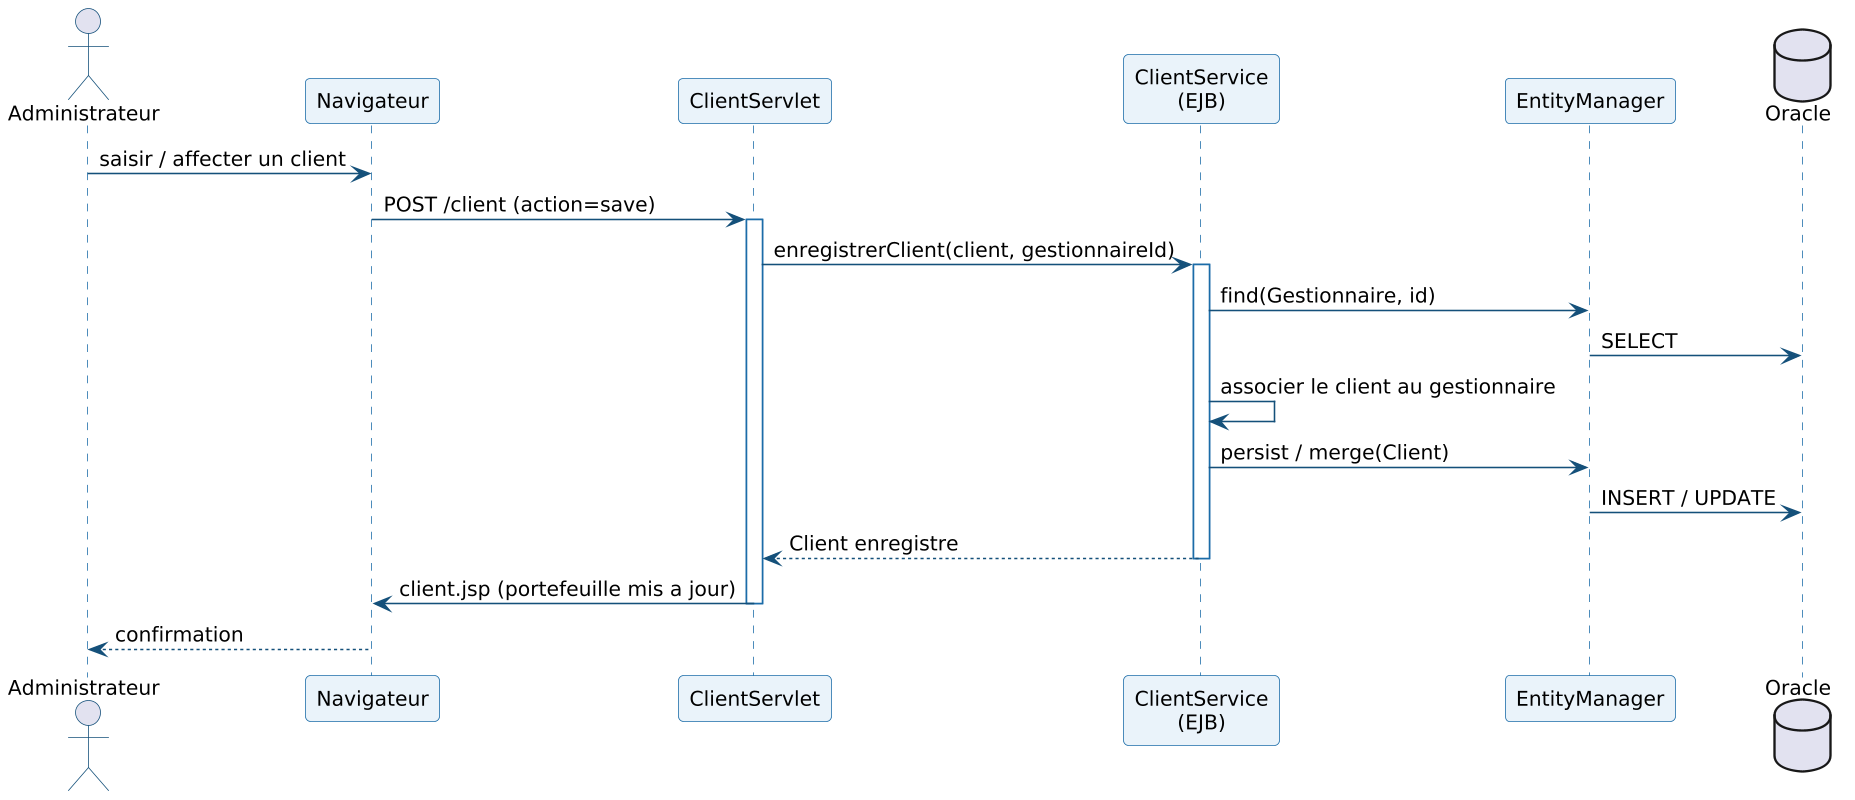
\includegraphics[width=0.92\textwidth]{seq_client.png}
  \caption{Diagramme de séquence -- Gestion d'un client}
  \label{fig:seq_client}
\end{figure}

Le \texttt{ClientServlet} transmet la demande au \texttt{ClientService}, qui
recherche le \texttt{Gestionnaire} concerné, associe le \texttt{Client} à ce
dernier, puis le persiste via l'\texttt{EntityManager}. Le portefeuille mis à jour
est renvoyé à la page \texttt{client.jsp}.

\section{Réalisation : interfaces utilisateur}
La figure~\ref{fig:ui_clients} illustre les interfaces de gestion des clients et
de suivi des objectifs. \emph{Les captures d'écran réelles seront insérées à cet
emplacement.}

\begin{figure}[htbp]
  \centering
  \fbox{\parbox[c][3.6cm][c]{0.8\textwidth}{\centering\itshape Capture à insérer
  -- gestion des clients et suivi des objectifs}}
  \caption{Interfaces de gestion des clients et des objectifs}
  \label{fig:ui_clients}
\end{figure}

\section*{Conclusion}
Ce sprint a complété la gestion commerciale (clients et objectifs). Le sprint
suivant aborde le pointage des employés, les workflows de demandes et les
notifications.
             % Ch.5 — Sprint 3 : Clients et objectifs
% ===================== CHAPITRE 6 — SPRINT 4 =========================
\chapter{Sprint 4 : Pointage, demandes et notifications}

\section*{Introduction}
Ce sprint regroupe trois mécanismes transverses : le \textbf{pointage} de présence
des employés, les \textbf{workflows de demandes} (création et modification) et le
dispositif de \textbf{notifications} et de \textbf{journalisation} des actions.

\section{Objectifs du Sprint}
L'objectif est d'assurer le \textbf{suivi de présence} des employés, d'\textbf{encadrer}
les opérations sensibles par des circuits de validation et de garantir la
\textbf{traçabilité} des actions par la journalisation et les notifications.

\section{Spécification des besoins}

\subsection{Diagramme de cas d'utilisation du Sprint 4}
La figure~\ref{fig:uc_s4} présente les cas d'utilisation du sprint.

\begin{figure}[htbp]
  \centering
  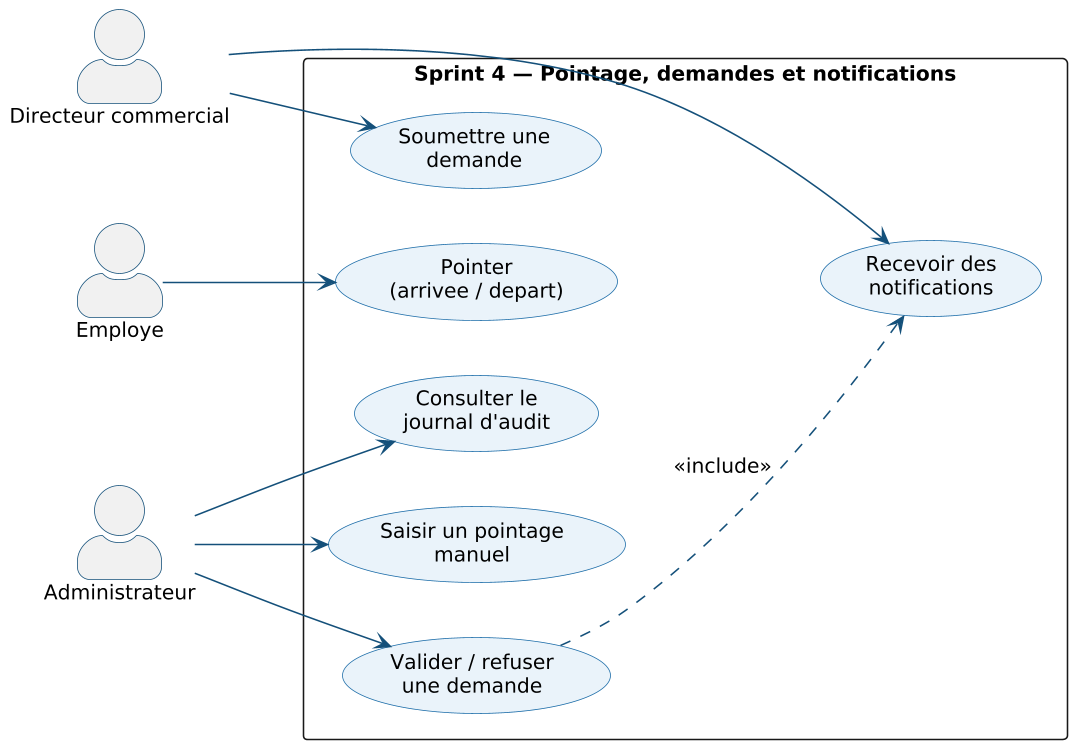
\includegraphics[width=0.92\textwidth]{uc_sprint4.png}
  \caption{Diagramme de cas d'utilisation du Sprint 4}
  \label{fig:uc_s4}
\end{figure}

\subsection{Sprint Backlog du sprint 4}
Le tableau~\ref{tab:bl_s4} détaille les user stories et les tâches techniques.

\begin{table}[htbp]
\centering
\caption{Sprint Backlog du sprint 4}
\label{tab:bl_s4}
\renewcommand{\arraystretch}{1.3}
\begin{tabularx}{\textwidth}{>{\bfseries}p{1cm}p{5cm}X}
\toprule
\textmd{\textbf{US}} & \textbf{User story} & \textbf{Tâches techniques}\\
\midrule
US9 & Pointer la présence (arrivée / départ). &
Développer l'entité \texttt{Pointage}, le \texttt{PointageService} (EJB) et le
\texttt{PointageServlet} (\texttt{/pointage}) ; déterminer le statut
(\texttt{PRESENT} / \texttt{RETARD} au-delà de 9h) ; page \texttt{pointage.jsp}.\\
\midrule
US10 & Saisir ou corriger un pointage manuel. &
Permettre à l'administrateur de saisir un pointage (\texttt{PRESENT},
\texttt{RETARD}, \texttt{ABSENT}) via \texttt{PointageService.saveManuel}.\\
\midrule
US11 & Soumettre une demande (client, employé, modification). &
Développer les entités \texttt{DemandeClient}, \texttt{DemandeEmploye},
\texttt{DemandeModification}, \texttt{DemandeAgence} et les servlets
\texttt{DemandeAgenceServlet} / \texttt{MesDemandesServlet} ; statut
\texttt{EN\_ATTENTE}.\\
\midrule
US12 & Valider ou refuser une demande. &
Développer le \texttt{GestionModificationsServlet} et le
\texttt{DemandeAgenceAdminServlet} ; faire évoluer le statut vers
\texttt{EFFECTUE} / \texttt{REFUSE} ; pages \texttt{gestion-demandes.jsp},
\texttt{demandes-admin.jsp}.\\
\midrule
US13 & Recevoir des notifications et consulter le journal d'audit. &
Développer le \texttt{NotificationService}, l'entité \texttt{Notification} et le
\texttt{NotificationFilter} ; journaliser les actions via le
\texttt{JournalService} (\texttt{JournalAction}).\\
\bottomrule
\end{tabularx}
\end{table}

\section{Analyse des besoins}

\subsection{Description textuelle des cas d'utilisation}

\cudesc{tab:cu_pointage}{Pointer la présence}
{Permettre à l'employé d'enregistrer son arrivée et son départ, avec
détermination automatique du statut.}
{Utilisateur (employé)}
{L'employé doit être authentifié.}
{Le pointage du jour est enregistré avec son statut (\texttt{PRESENT} ou
\texttt{RETARD}).}
{(1) L'employé clique sur « Pointer » ; (2) le \texttt{PointageService} relève
l'heure courante et recherche le pointage du jour ; (3) s'il n'existe pas, il
détermine le statut (\texttt{RETARD} au-delà de 9h) et l'enregistre ; (4) sinon,
il met à jour l'enregistrement existant.}

\cudesc{tab:cu_demande}{Valider une demande}
{Permettre à l'administrateur d'approuver ou de refuser une demande soumise.}
{Administrateur}
{Une demande au statut \texttt{EN\_ATTENTE} doit exister.}
{Le statut de la demande évolue vers \texttt{EFFECTUE} ou \texttt{REFUSE} et
l'action est journalisée.}
{(1) L'administrateur consulte les demandes en attente ; (2) il sélectionne une
demande ; (3) il l'approuve ou la refuse avec un commentaire ; (4) le service met
à jour le statut, applique la modification le cas échéant et journalise l'action.}

\section{Conception}

\subsection{Diagramme de séquence : « Pointer un employé »}
La figure~\ref{fig:seq_pointage} décrit le scénario de pointage.

\begin{figure}[htbp]
  \centering
  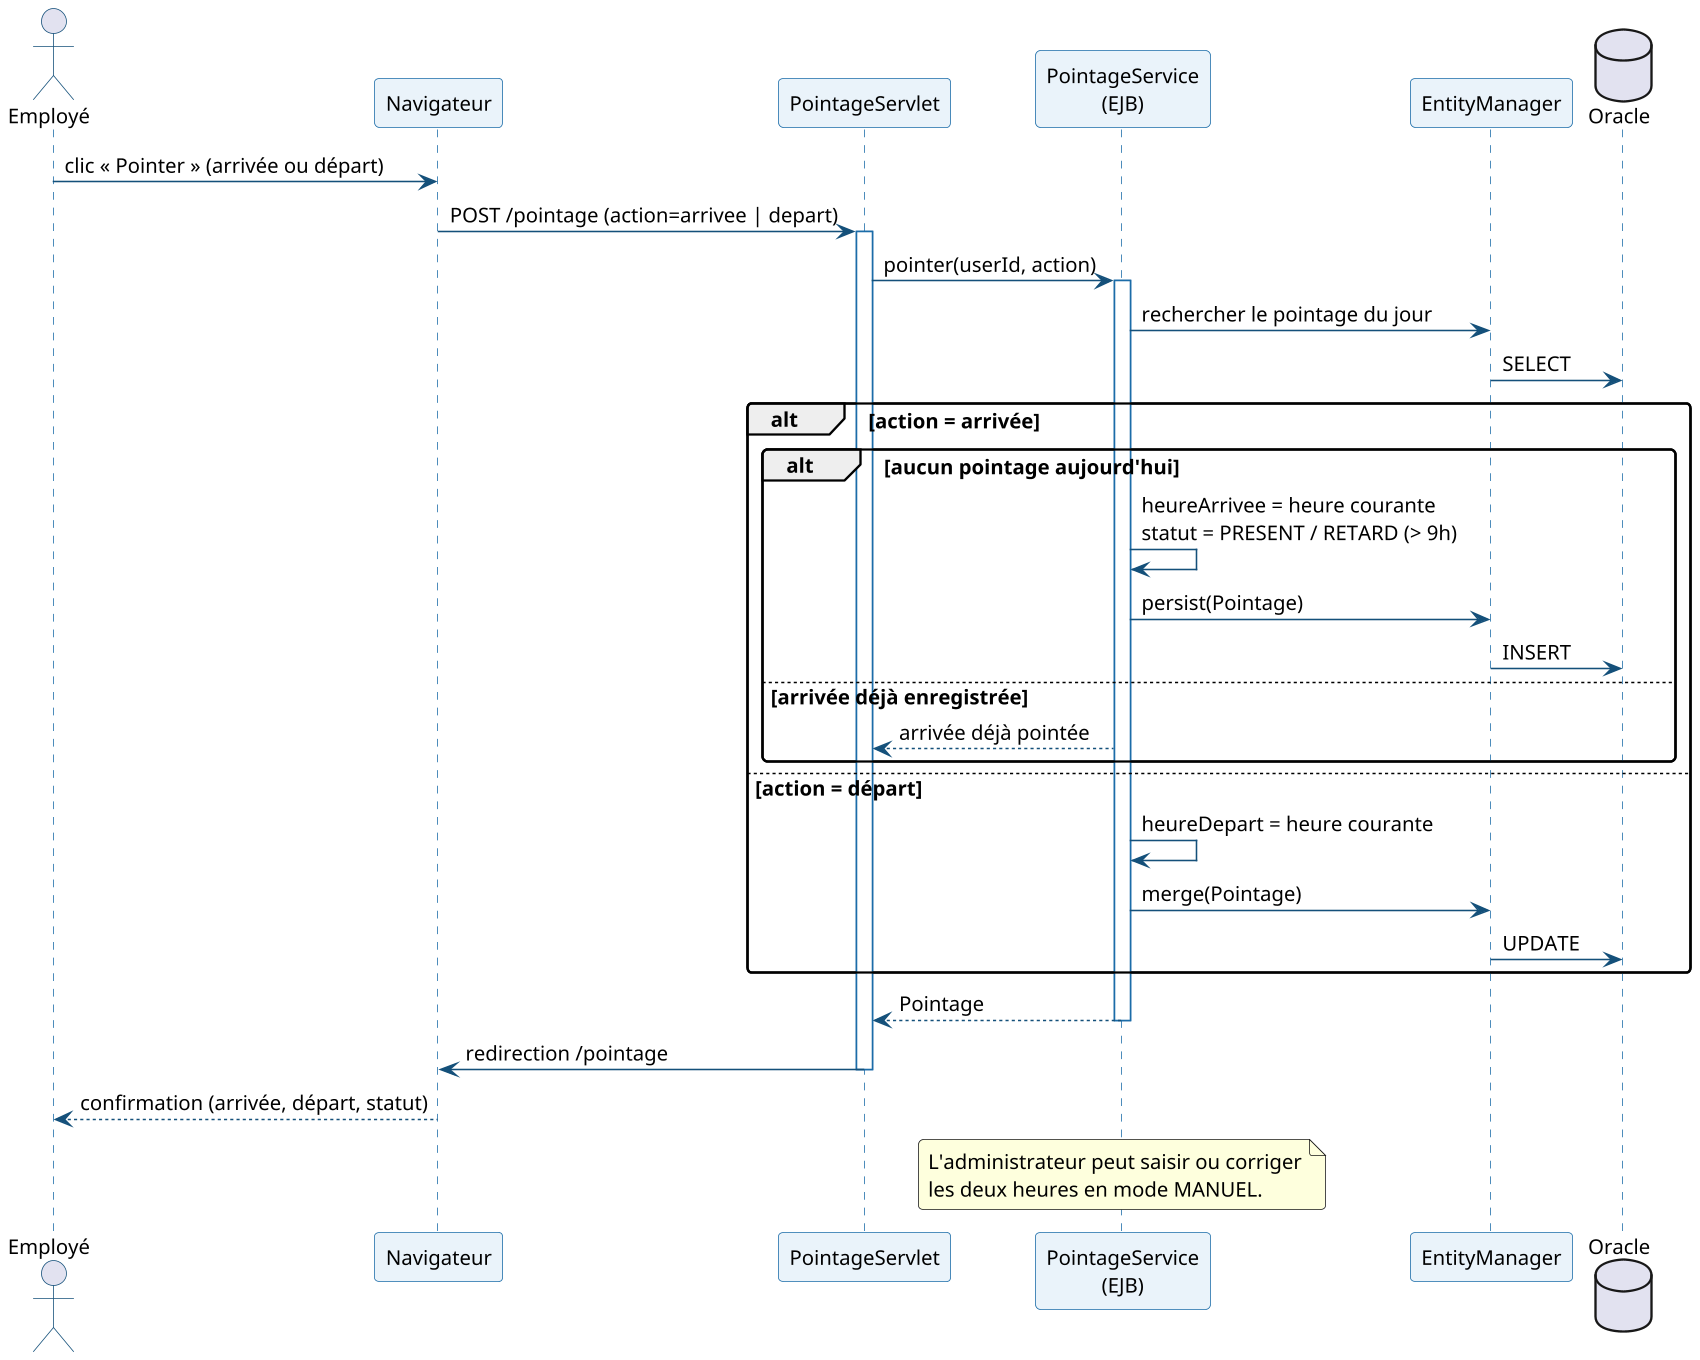
\includegraphics[width=0.95\textwidth]{seq_pointage.png}
  \caption{Diagramme de séquence -- Pointage d'un employé}
  \label{fig:seq_pointage}
\end{figure}

Le \texttt{PointageServlet} transmet l'action au \texttt{PointageService}, qui
recherche le pointage du jour. Le fragment \texttt{alt} distingue l'\texttt{INSERT}
(premier pointage, statut \texttt{PRESENT}/\texttt{RETARD} au-delà de 9h) de
l'\texttt{UPDATE} (pointage déjà existant).

\subsection{Diagramme de séquence : « Valider une demande »}
La figure~\ref{fig:seq_demande} détaille le traitement d'une demande par
l'administrateur.

\begin{figure}[htbp]
  \centering
  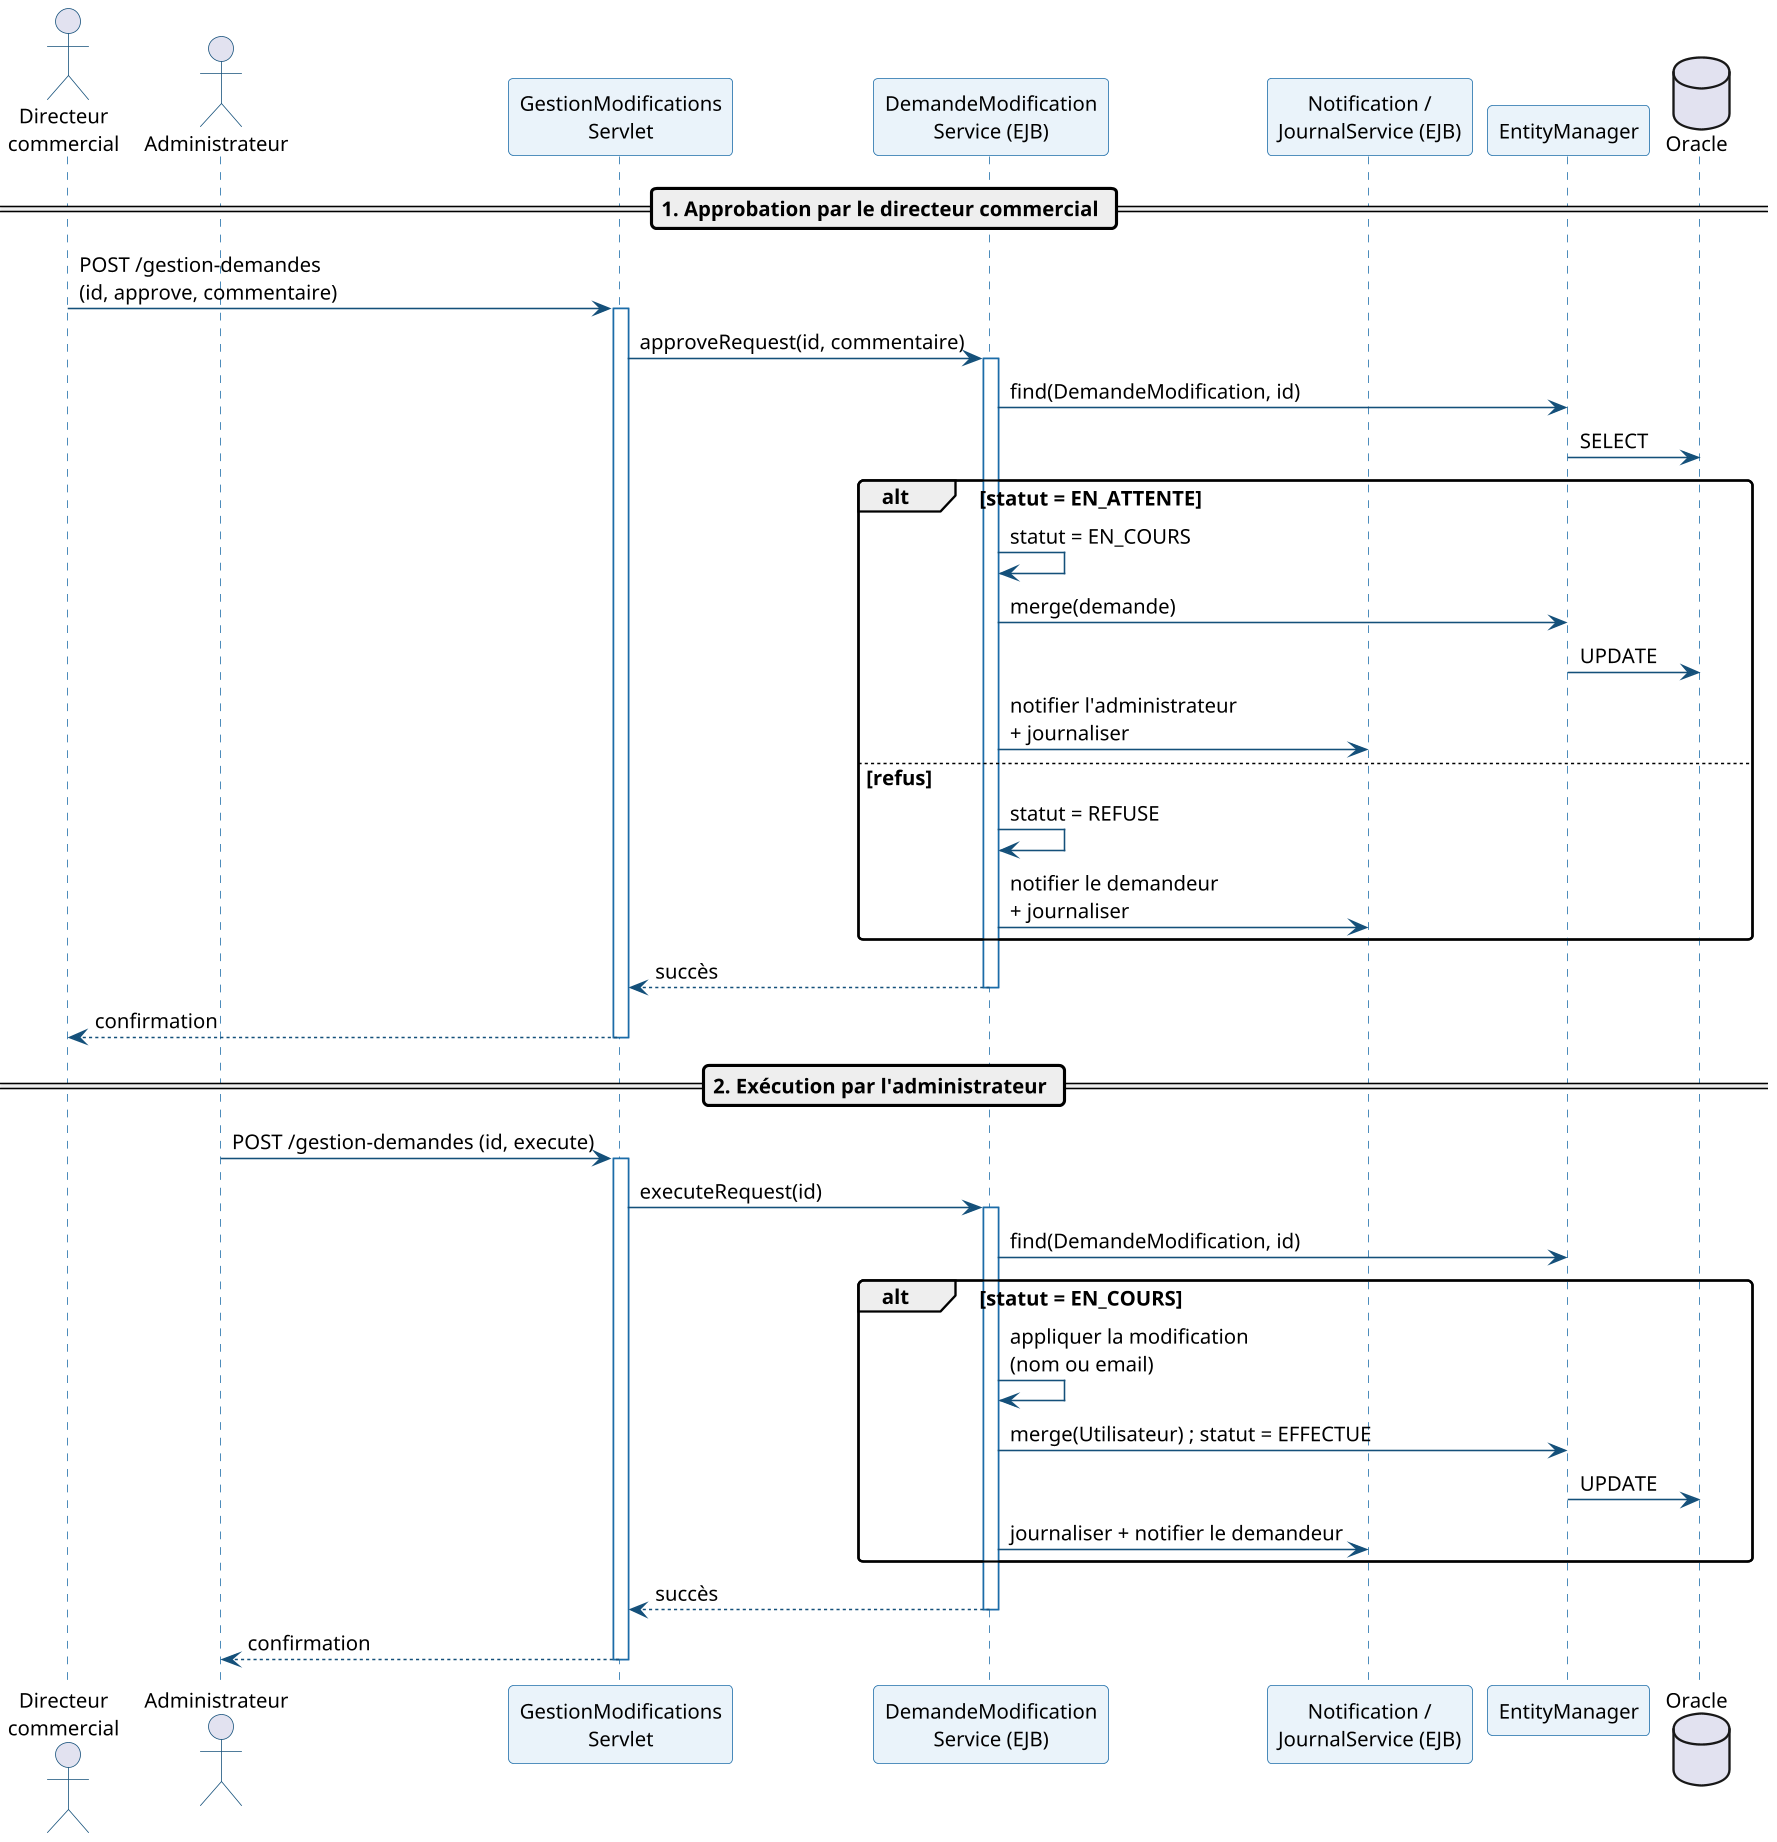
\includegraphics[width=0.92\textwidth]{seq_demande.png}
  \caption{Diagramme de séquence -- Validation d'une demande}
  \label{fig:seq_demande}
\end{figure}

Le \texttt{GestionModificationsServlet} transmet la décision au service métier,
qui charge la demande, met à jour son statut, persiste la modification puis
journalise l'action via le \texttt{JournalService}.

\subsection{Diagramme d'états-transitions : cycle de vie d'une demande}
La figure~\ref{fig:state_demande} modélise le cycle de vie d'une demande.

\begin{figure}[htbp]
  \centering
  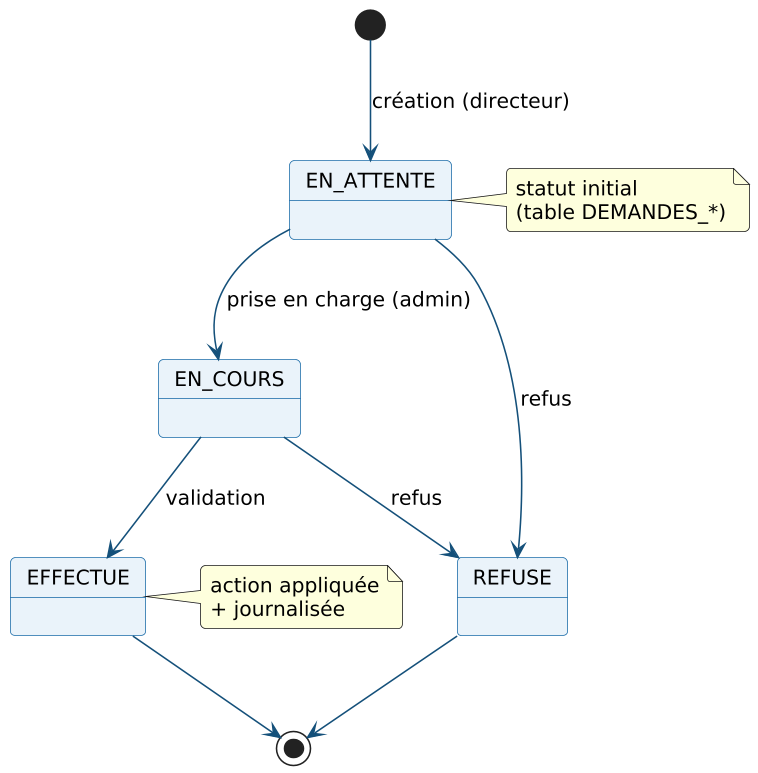
\includegraphics[width=0.6\textwidth]{state_demande.png}
  \caption{Diagramme d'états-transitions -- Cycle de vie d'une demande}
  \label{fig:state_demande}
\end{figure}

Une demande naît à l'état \texttt{EN\_ATTENTE}, passe en \texttt{EN\_COURS} lors de
sa prise en charge, puis atteint un état final \texttt{EFFECTUE} ou
\texttt{REFUSE}, en cohérence avec la contrainte de la table des demandes.

\subsection{Diagramme d'activité : traitement d'une demande}
La figure~\ref{fig:activity_demande} représente le processus métier de traitement
d'une demande.

\begin{figure}[htbp]
  \centering
  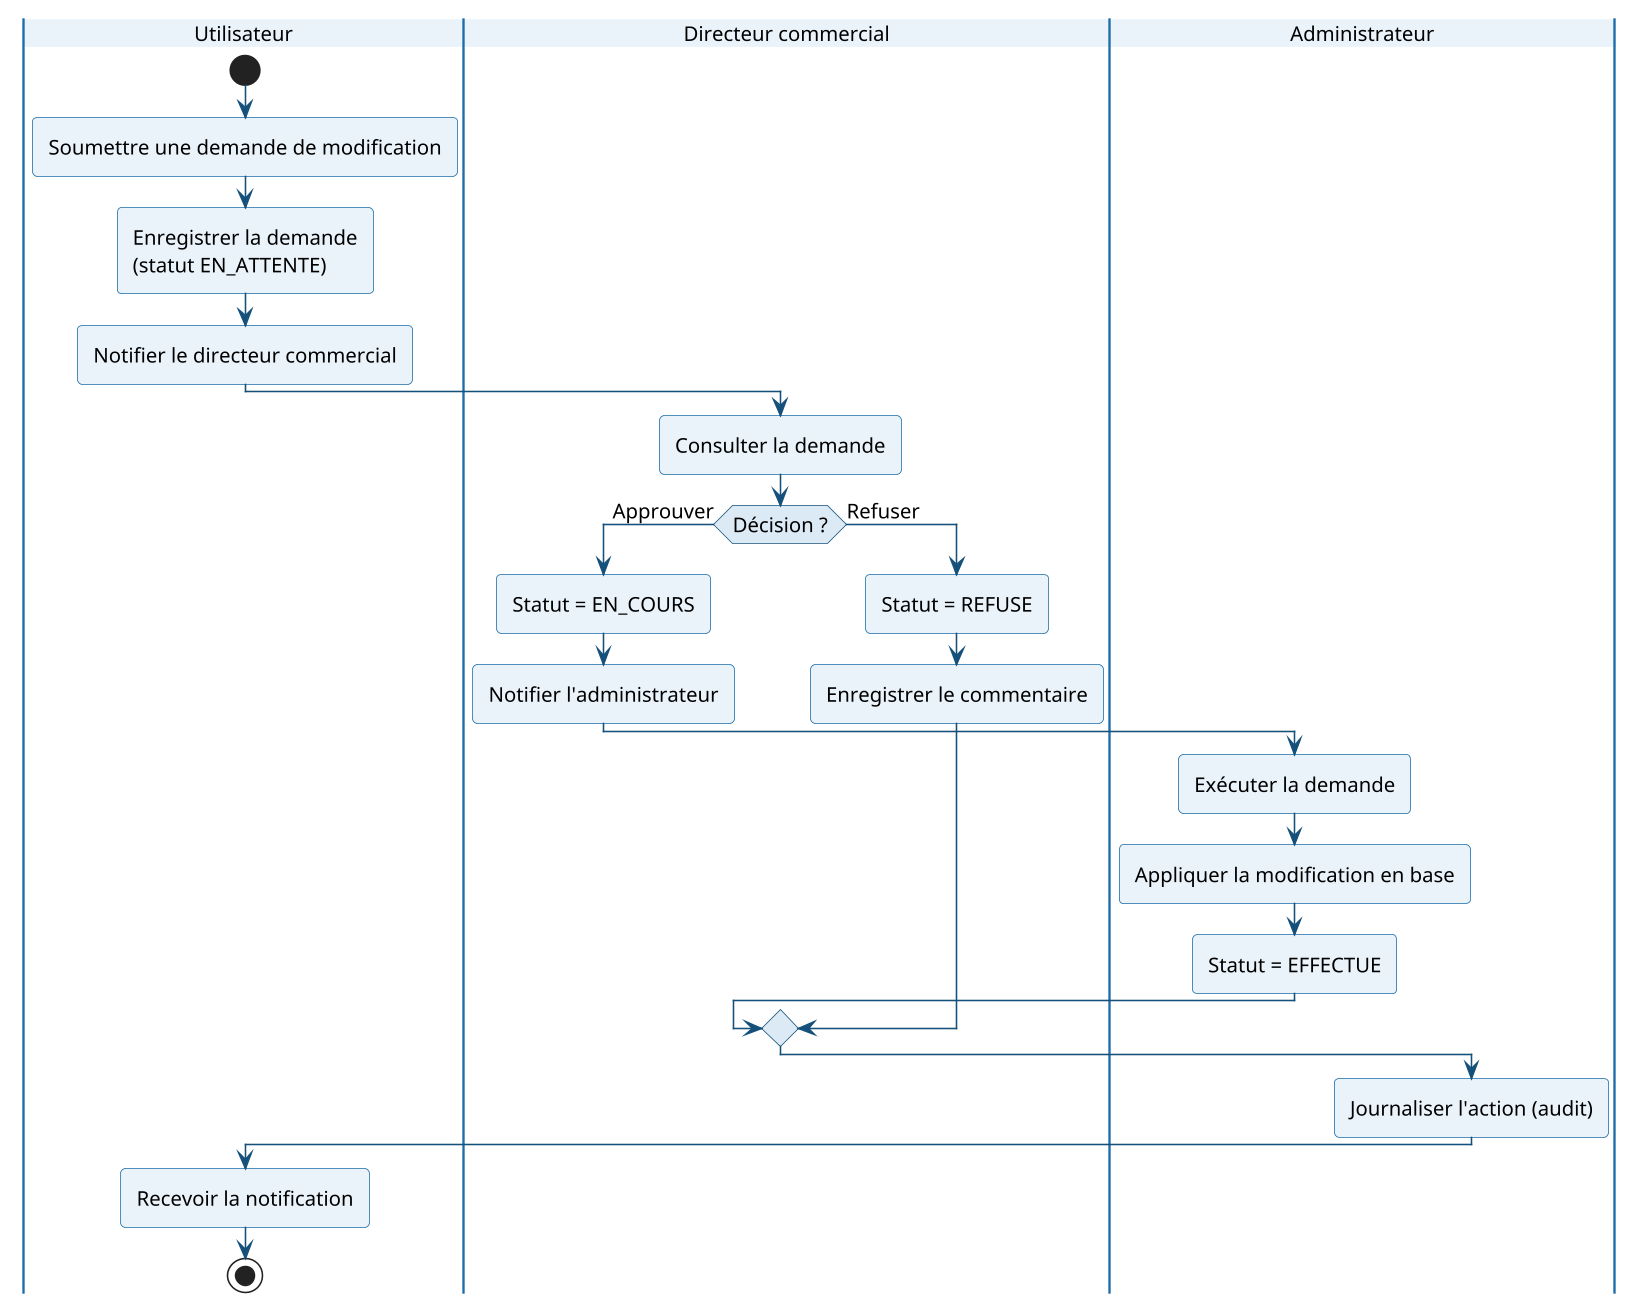
\includegraphics[width=0.6\textwidth]{activity_demande.png}
  \caption{Diagramme d'activité -- Traitement d'une demande}
  \label{fig:activity_demande}
\end{figure}

Le directeur soumet une demande, notifiée à l'administrateur. Le nœud de décision
oriente le flux : en cas de validation, le statut passe à \texttt{EFFECTUE} et la
modification est appliquée ; en cas de refus, le statut passe à \texttt{REFUSE}
avec un commentaire. Les deux branches convergent vers la journalisation et la
notification du demandeur.

\section{Réalisation : interfaces utilisateur}
La figure~\ref{fig:ui_pointage} présente l'interface du module de pointage : les
cartes de synthèse (présents, retards, absents, taux de présence), le pointage du
jour (boutons « Pointer l'arrivée / le départ ») et le formulaire de saisie ou de
correction manuelle.

\begin{figure}[htbp]
  \centering
  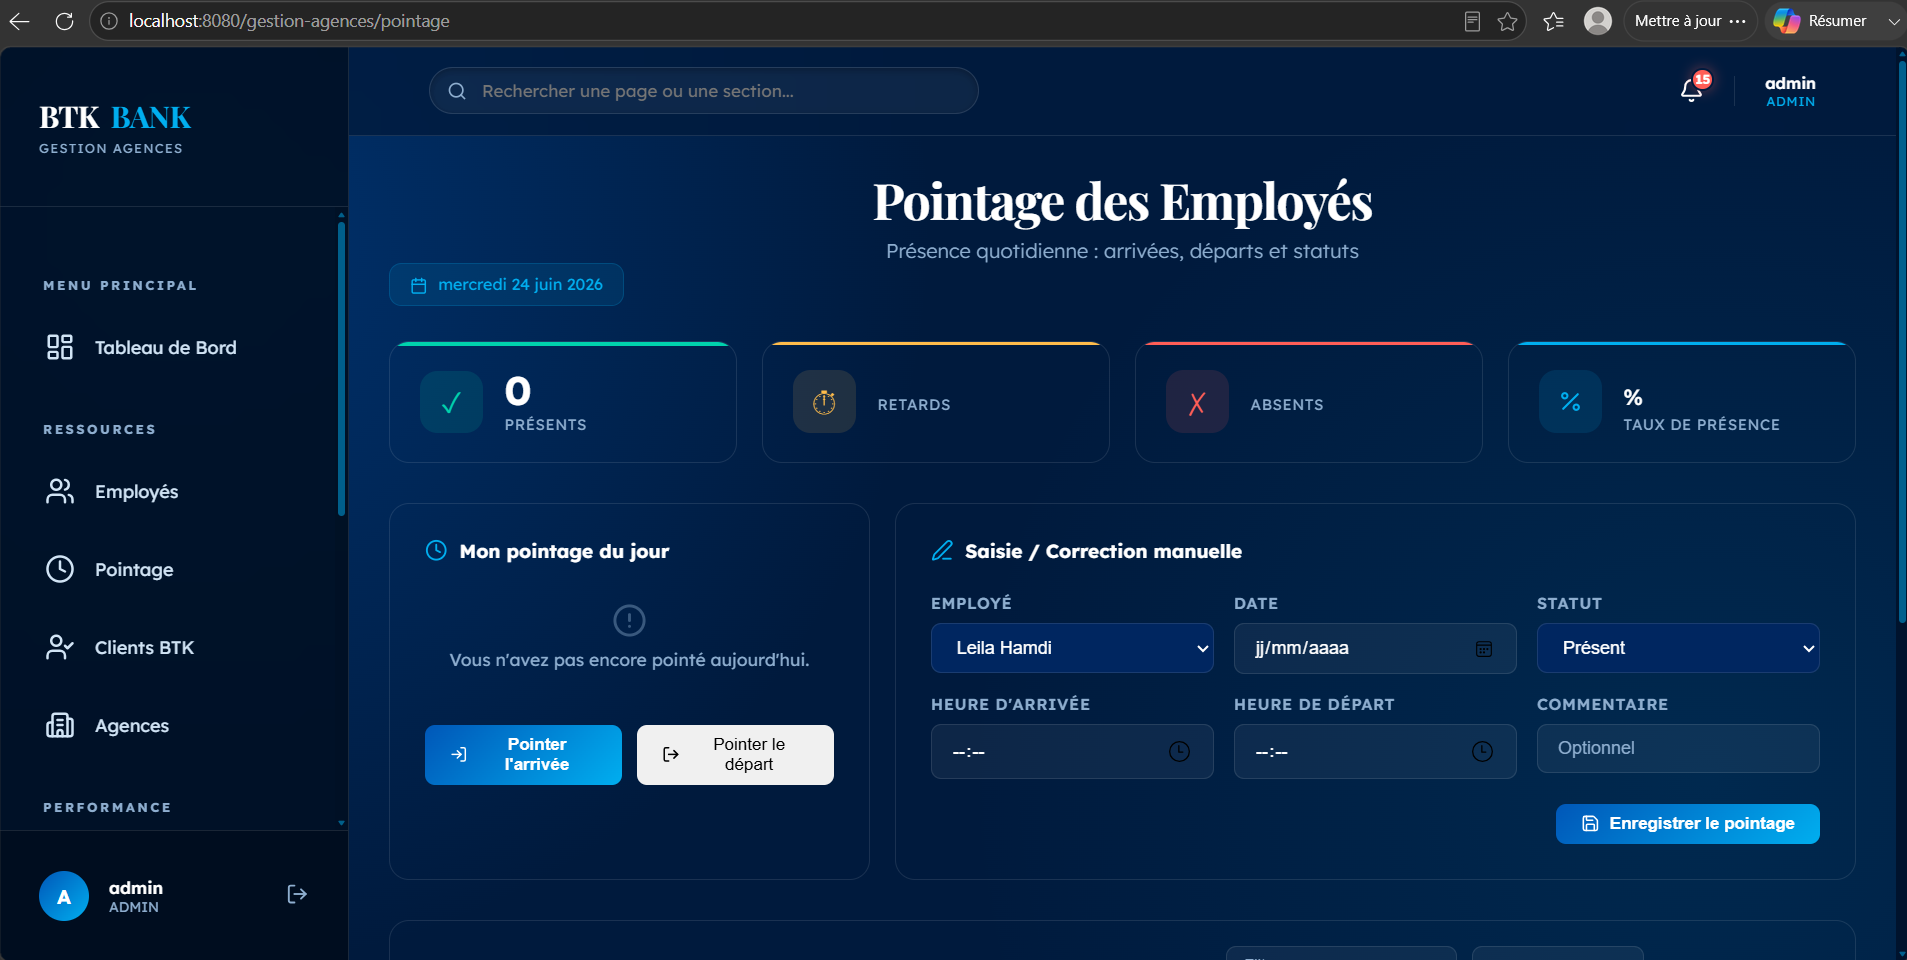
\includegraphics[width=\textwidth]{screens/pointage.png}
  \caption{Interface du module de pointage des employés}
  \label{fig:ui_pointage}
\end{figure}

\section*{Conclusion}
Ce sprint a doté l'application du suivi de présence, des circuits de validation et
de la traçabilité des actions. Le sprint suivant met en place la chaîne ETL et le
volet décisionnel.
             % Ch.6 — Sprint 4 : Pointage et demandes
% ===================== CHAPITRE 7 — SPRINT 5 =========================
\chapter{Sprint 5 : Chaîne ETL et volet décisionnel}

\section*{Introduction}
Ce sprint réalise le \textbf{volet décisionnel} de la solution. Il met en place
une chaîne \textbf{ETL} qui consolide les données opérationnelles dans un
\textbf{datamart}, puis restitue les indicateurs au moyen d'un tableau de bord
embarqué et de rapports Power BI.

\section{Objectifs du Sprint}
L'objectif est de \textbf{consolider} les données dispersées (employés, clients,
objectifs, pointage) en un datamart agrégé par agence, et de \textbf{restituer}
les indicateurs de pilotage aux responsables.

\section{Spécification des besoins}

\subsection{Diagramme de cas d'utilisation du Sprint 5}
La figure~\ref{fig:uc_s5} présente les cas d'utilisation du sprint.

\begin{figure}[htbp]
  \centering
  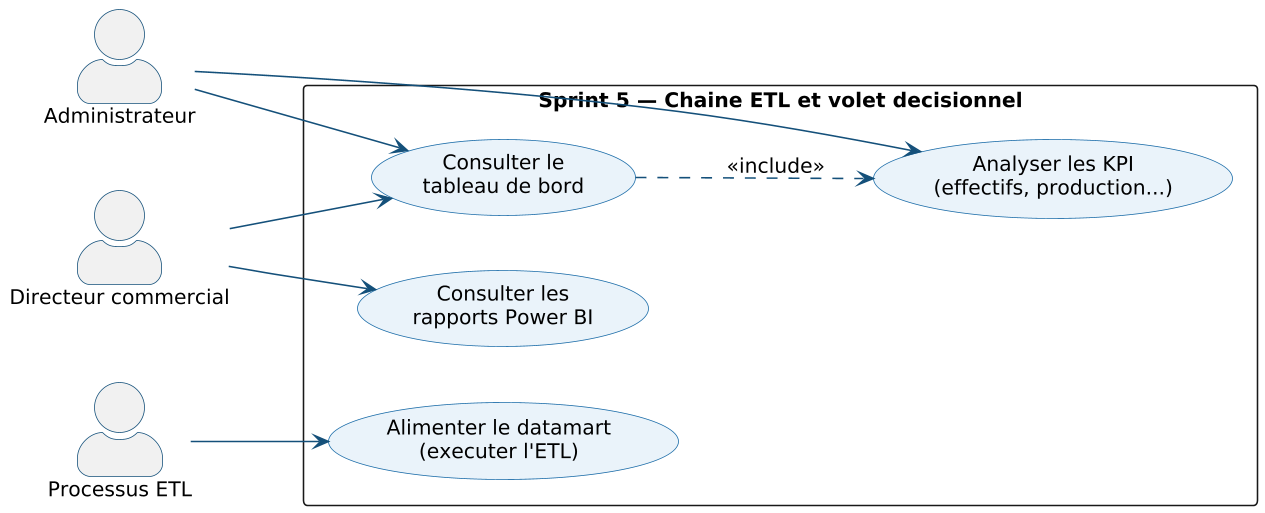
\includegraphics[width=0.86\textwidth]{uc_sprint5.png}
  \caption{Diagramme de cas d'utilisation du Sprint 5}
  \label{fig:uc_s5}
\end{figure}

\subsection{Sprint Backlog du sprint 5}
Le tableau~\ref{tab:bl_s5} détaille les user stories et les tâches techniques.

\begin{table}[htbp]
\centering
\caption{Sprint Backlog du sprint 5}
\label{tab:bl_s5}
\renewcommand{\arraystretch}{1.3}
\begin{tabularx}{\textwidth}{>{\bfseries}p{1cm}p{5cm}X}
\toprule
\textmd{\textbf{US}} & \textbf{User story} & \textbf{Tâches techniques}\\
\midrule
US14 & Alimenter le datamart via la chaîne ETL. &
Développer le script Python \texttt{etl\_agences.py} (pandas) ; étapes
\emph{Extract / Transform / Load} ; agréger les indicateurs par agence ; produire
le datamart en étoile (\texttt{dim\_agence}, \texttt{fait\_agence}).\\
\midrule
US15 & Consulter le tableau de bord décisionnel. &
Enrichir le \texttt{HomeServlet} avec les statistiques ; réaliser le tableau de
bord \texttt{home.jsp} (cartes d'indicateurs et graphiques ApexCharts).\\
\midrule
US16 & Consulter les rapports Power BI. &
Créer les vues analytiques \texttt{V\_BI\_EMPLOYES}, \texttt{V\_BI\_CLIENTS},
\texttt{V\_BI\_OBJECTIFS}, \texttt{V\_BI\_POINTAGE} ; les connecter à Power BI.\\
\bottomrule
\end{tabularx}
\end{table}

\section{Analyse des besoins}

\subsection{Description textuelle des cas d'utilisation}

\cudesc{tab:cu_etl}{Alimenter le datamart (ETL)}
{Consolider les données opérationnelles en un datamart agrégé par agence.}
{Processus ETL / Administrateur}
{Les données sources (agences, employés, clients, objectifs, pointage) doivent
être disponibles.}
{Le datamart en étoile est produit et mis à la disposition de la restitution et de
la segmentation.}
{(1) L'étape \emph{Extract} lit les données sources ; (2) l'étape \emph{Transform}
les nettoie et les agrège par agence ; (3) l'étape \emph{Load} écrit le datamart
(\texttt{dim\_agence}, \texttt{fait\_agence}).}

\cudesc{tab:cu_dashboard}{Consulter le tableau de bord}
{Restituer aux responsables une vision synthétique de l'activité.}
{Administrateur / Directeur commercial}
{L'acteur doit être authentifié.}
{Les indicateurs clés (effectifs, présence, production) sont affichés.}
{(1) L'acteur se connecte ; (2) le \texttt{HomeServlet} calcule les statistiques ;
(3) la page \texttt{home.jsp} affiche les cartes d'indicateurs et les graphiques
ApexCharts.}

\section{Conception}

\subsection{Chaîne décisionnelle et processus ETL}
Les données nécessaires au pilotage sont dispersées dans les tables opérationnelles
et exprimées à des grains hétérogènes. Le processus \textbf{ETL} (\emph{Extract --
Transform -- Load}) les consolide en un datamart agrégé par agence. La
figure~\ref{fig:etl_chaine} présente cette chaîne décisionnelle.

\begin{figure}[htbp]
  \centering
  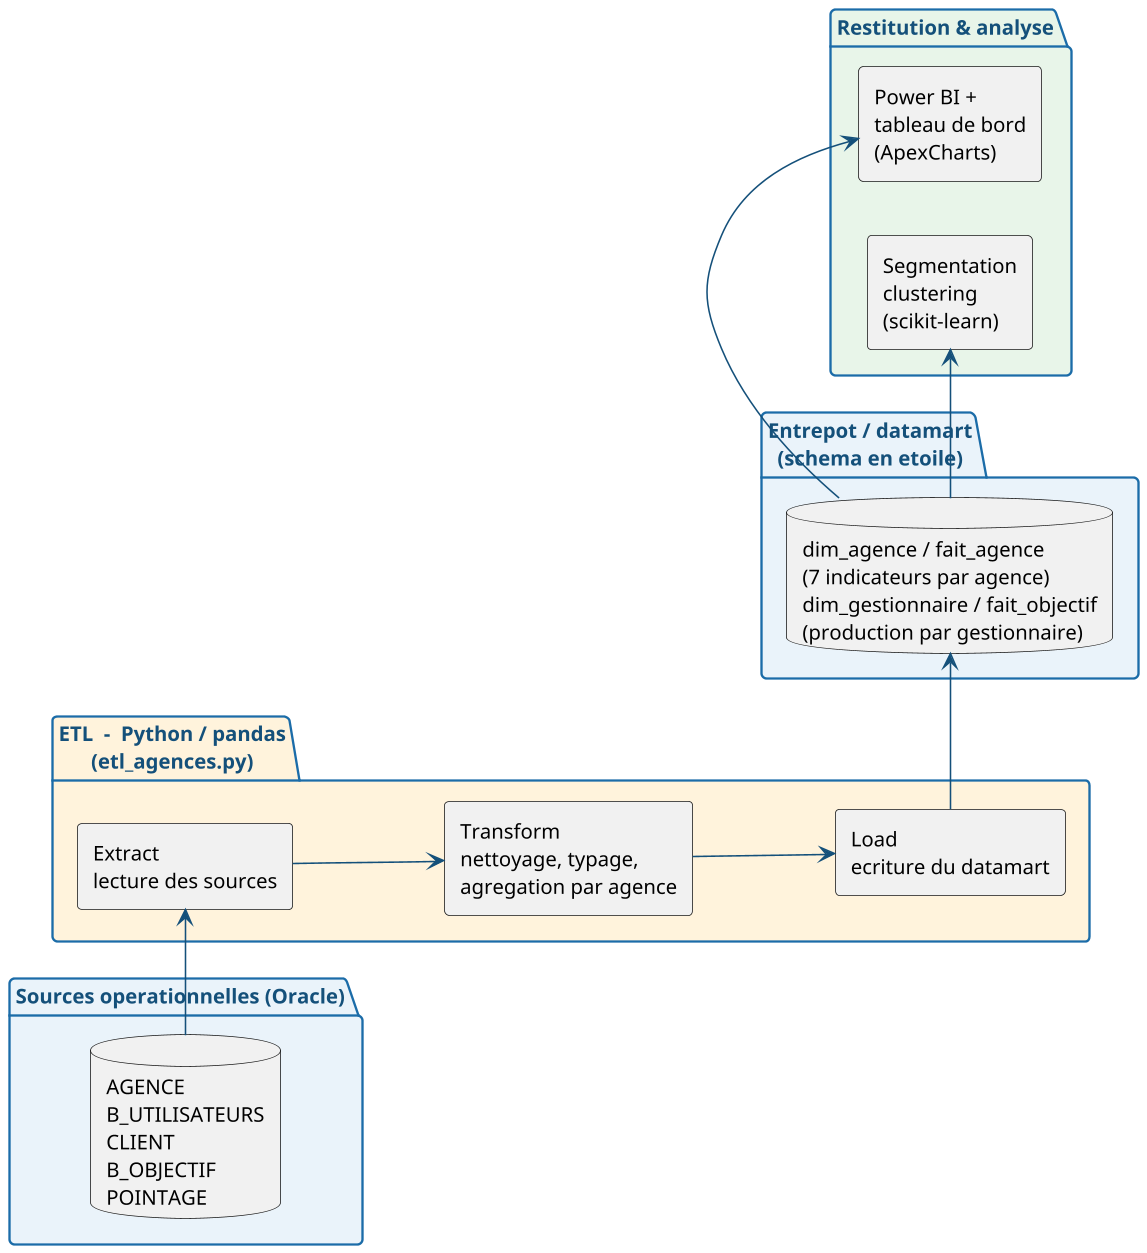
\includegraphics[width=\textwidth]{etl_chaine.png}
  \caption{Chaîne décisionnelle : du système opérationnel au datamart et à sa restitution}
  \label{fig:etl_chaine}
\end{figure}

Trois étapes s'enchaînent : \textbf{Extract} (lecture des sources
\texttt{AGENCE}, \texttt{B\_UTILISATEURS}, \texttt{CLIENT}, \texttt{B\_OBJECTIF},
\texttt{POINTAGE}), \textbf{Transform} (nettoyage, typage et agrégation par agence)
et \textbf{Load} (chargement du datamart en étoile). Ce datamart constitue une
\textbf{source unique consolidée}, partagée par la restitution (tableau de bord et
Power BI) et par la segmentation des agences (chapitre~\ref{chap:segmentation}).

\subsection{Modèle en étoile de l'entrepôt}
L'entrepôt est organisé selon une logique en \textbf{étoile}
(figure~\ref{fig:bi}) : autour de tables de faits (production, effectifs, clients,
présence), des dimensions descriptives (agence, gestionnaire, période, type de
client) permettent l'analyse multidimensionnelle. Les vues \texttt{V\_BI\_*}
matérialisent cette couche sémantique pour l'outil de restitution.

\begin{figure}[htbp]
  \centering
  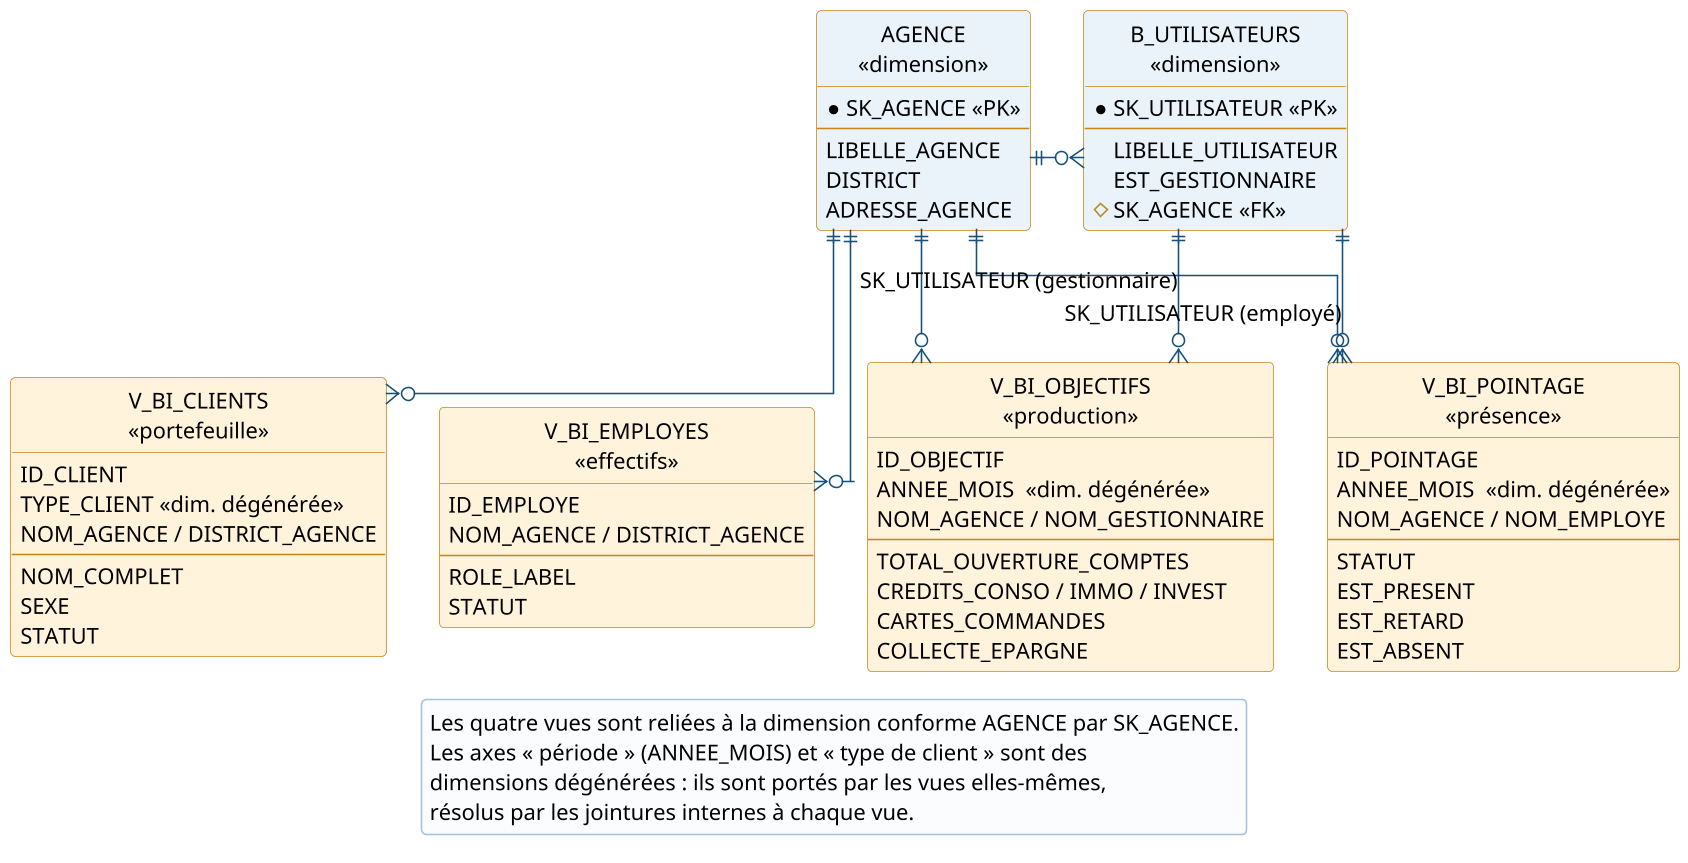
\includegraphics[width=0.95\textwidth]{bi.png}
  \caption{Modèle décisionnel en étoile (vues \texttt{V\_BI\_*})}
  \label{fig:bi}
\end{figure}

Le tableau~\ref{tab:kpi} récapitule les principaux indicateurs (KPI) retenus.

\begin{table}[htbp]
\centering
\caption{Indicateurs de performance (KPI) du volet décisionnel}
\label{tab:kpi}
\renewcommand{\arraystretch}{1.25}
\begin{tabularx}{\textwidth}{>{\bfseries}p{4.2cm}Xp{2.6cm}}
\toprule
\textmd{\textbf{Indicateur}} & \textbf{Description} & \textbf{Source}\\
\midrule
Effectifs par agence & Nombre d'employés par agence & \texttt{V\_BI\_EMPLOYES}\\
Répartition des rôles & Gestionnaires / conseillers / hors commercial & \texttt{V\_BI\_EMPLOYES}\\
Portefeuille clients & Clients par type et par agence & \texttt{V\_BI\_CLIENTS}\\
Ouvertures de comptes & Comptes chèques + épargne + courants & \texttt{V\_BI\_OBJECTIFS}\\
Production de crédits & Conso, immobilier, investissement & \texttt{V\_BI\_OBJECTIFS}\\
Collecte d'épargne & Épargne additionnelle collectée & \texttt{V\_BI\_OBJECTIFS}\\
Taux de présence & Présents, retards et absences par agence et période & \texttt{V\_BI\_POINTAGE}\\
\bottomrule
\end{tabularx}
\end{table}

\section{Réalisation}

\subsection{Mise en œuvre de la chaîne ETL en Python}
La chaîne ETL est implémentée en \textbf{Python} (script \texttt{etl\_agences.py})
à l'aide de la bibliothèque \textbf{pandas}~\cite{pandas}. Elle est organisée en
trois fonctions : \texttt{extract()} lit les données sources (connexion Oracle via
le connecteur \texttt{oracledb} ou, à défaut, export CSV) ; \texttt{transform()}
nettoie et \textbf{agrège les données par agence} pour produire les sept
indicateurs de pilotage ; \texttt{load()} écrit le datamart en étoile
(\texttt{dim\_agence}, \texttt{fait\_agence}) et le fichier réutilisé par la
segmentation. L'extrait~\ref{lst:etl_transform} illustre le cœur de l'agrégation.

\begin{lstlisting}[style=pycode,caption={Agrégation des indicateurs par agence (étape Transform)},label={lst:etl_transform}]
# effectif et nombre de gestionnaires par agence
eff = employes.groupby("SK_AGENCE").agg(
    effectif=("SK_UTILISATEUR", "count"),
    nb_gestionnaires=("EST_GESTIONNAIRE", "sum")).reset_index()
# portefeuille clients
cli = clients.groupby("SK_AGENCE").size().reset_index(name="nb_clients")
# production (comptes, credits, epargne)
obj = objectifs.groupby("SK_AGENCE").agg(
    total_comptes=("COMPTES", "sum"),
    production_credits=("CREDITS", "sum"),
    collecte_epargne=("EPARGNE", "sum")).reset_index()
# taux de presence issu du pointage
poi = pointages.assign(
        present=pointages["STATUT"].isin(["PRESENT", "RETARD"]).astype(int)) \
    .groupby("SK_AGENCE").agg(taux_presence=("present", "mean")).reset_index()
\end{lstlisting}

L'exécution du script produit le datamart sous \texttt{etl/entrepot/}
(\texttt{dim\_agence.csv}, \texttt{fait\_agence.csv}) ainsi que le fichier
consolidé \texttt{clustering/data/agences.csv}. Le pipeline est \textbf{rejouable}
et journalise le nombre d'enregistrements traités à chaque étape.

\subsection{Tableau de bord et restitution Power BI}
Le tableau de bord embarqué (\texttt{home.jsp}, alimenté par le
\texttt{HomeServlet}) comporte une rangée de \textbf{cartes d'indicateurs}
(employés, clients, présents du jour, taux de présence, demandes en attente) puis
des \textbf{graphiques} ApexCharts (effectif par agence, répartition des rôles,
présence du jour). En complément, les vues \texttt{V\_BI\_*} sont connectées à
\textbf{Power BI} pour des rapports interactifs. La figure~\ref{fig:ui_dashboard}
en présente les interfaces. \emph{Les captures d'écran réelles seront insérées à
cet emplacement.}

\begin{figure}[htbp]
  \centering
  \fbox{\parbox[c][3.6cm][c]{0.8\textwidth}{\centering\itshape Capture à insérer
  -- tableau de bord et rapport Power BI}}
  \caption{Tableau de bord embarqué et rapport Power BI}
  \label{fig:ui_dashboard}
\end{figure}

\section*{Conclusion}
Ce sprint a doté la solution d'un volet décisionnel complet : une chaîne ETL
alimente un datamart consolidé, restitué par un tableau de bord et par Power BI.
Le datamart ainsi produit constitue l'entrée du dernier sprint, consacré à la
segmentation des agences par apprentissage automatique.
             % Ch.7 — Sprint 5 : ETL et décisionnel
% ===================== CHAPITRE 8 — SPRINT 6 =========================
\chapter{Sprint 6 : Segmentation des agences par apprentissage non supervisé}
\label{chap:segmentation}

\section*{Introduction}
Ce dernier sprint introduit une brique d'\textbf{intelligence artificielle} : la
segmentation des agences par \textbf{apprentissage non supervisé}
(\emph{clustering}). À partir du datamart produit par la chaîne ETL, il regroupe
automatiquement les agences en profils homogènes afin d'éclairer les décisions de
pilotage.

\section{Objectifs du Sprint}
L'objectif est de \textbf{segmenter les agences} présentant des caractéristiques
d'activité similaires, sans étiquette préalable, afin d'appuyer le ciblage,
l'allocation des ressources et la définition d'objectifs différenciés.

\section{Spécification des besoins}

\subsection{Diagramme de cas d'utilisation du Sprint 6}
La figure~\ref{fig:uc_s6} présente les cas d'utilisation du sprint.

\begin{figure}[htbp]
  \centering
  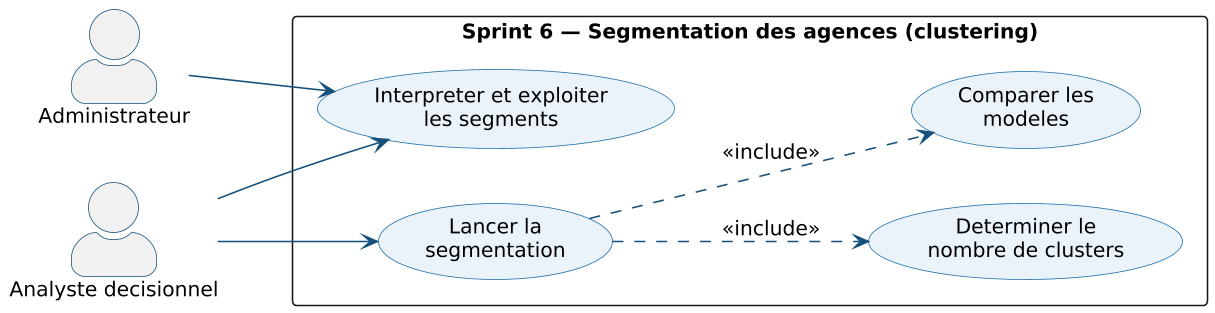
\includegraphics[width=0.82\textwidth]{uc_sprint6.png}
  \caption{Diagramme de cas d'utilisation du Sprint 6}
  \label{fig:uc_s6}
\end{figure}

\subsection{Sprint Backlog du sprint 6}
Le tableau~\ref{tab:bl_s6} détaille la user story et les tâches techniques.

\begin{table}[htbp]
\centering
\caption{Sprint Backlog du sprint 6}
\label{tab:bl_s6}
\renewcommand{\arraystretch}{1.3}
\begin{tabularx}{\textwidth}{>{\bfseries}p{1cm}p{4.4cm}X}
\toprule
\textmd{\textbf{US}} & \textbf{User story} & \textbf{Tâches techniques}\\
\midrule
US17 & Segmenter les agences par apprentissage non supervisé. &
Développer le script \texttt{segmentation\_agences.py} (scikit-learn) ; charger le
datamart et \textbf{standardiser} les variables ; déterminer le \textbf{nombre de
clusters} (coude + silhouette) ; \textbf{comparer} plusieurs modèles ; projeter en
\textbf{PCA} et \textbf{profiler} les segments.\\
\bottomrule
\end{tabularx}
\end{table}

\section{Analyse des besoins}

\subsection{Description textuelle du cas d'utilisation}

\cudesc{tab:cu_clustering}{Segmenter les agences}
{Regrouper automatiquement les agences en profils homogènes à partir de leurs
indicateurs d'activité.}
{Analyste décisionnel / Administrateur}
{Le datamart agrégé par agence (\texttt{fait\_agence}) doit être disponible.}
{Les agences sont réparties en segments cohérents, caractérisés et exploitables
pour la décision.}
{(1) L'analyste lance la segmentation ; (2) le script standardise les variables ;
(3) il détermine le nombre de clusters puis compare les modèles ; (4) il retient
le meilleur modèle, projette en PCA et restitue le profil de chaque segment.}

\section{Conception : démarche de clustering}

\subsection{Données et variables}
Les données ne sont pas extraites directement de la base opérationnelle : elles
proviennent du \textbf{datamart} produit par la chaîne ETL (table de faits
\texttt{fait\_agence}). Chaque agence y est décrite par sept indicateurs agrégés
(tableau~\ref{tab:variables_clustering}), ce qui garantit la cohérence entre le
tableau de bord, Power BI et l'analyse non supervisée.

\begin{table}[htbp]
\centering
\caption{Variables de segmentation (par agence)}
\label{tab:variables_clustering}
\renewcommand{\arraystretch}{1.2}
\begin{tabularx}{\textwidth}{>{\bfseries}p{4cm}X}
\toprule
\textmd{\textbf{Variable}} & \textbf{Description}\\
\midrule
effectif & Nombre d'employés de l'agence\\
nb\_gestionnaires & Nombre de gestionnaires\\
nb\_clients & Taille du portefeuille clients\\
total\_comptes & Total des ouvertures de comptes\\
production\_credits & Production de crédits\\
collecte\_epargne & Collecte d'épargne\\
taux\_presence & Taux de présence (issu du pointage)\\
\bottomrule
\end{tabularx}
\end{table}

\subsection{Prétraitement}
Les variables étant exprimées dans des ordres de grandeur très différents (un
effectif de quelques dizaines face à des milliers de comptes), une
\textbf{standardisation} (centrage-réduction, \texttt{StandardScaler}) est
appliquée. Sans elle, les variables de forte amplitude domineraient le calcul des
distances et fausseraient le regroupement.

\subsection{Détermination du nombre de clusters}
Le nombre de clusters $k$ étant inconnu a priori, il est déterminé en combinant la
\textbf{méthode du coude} (inertie intra-cluster) et le \textbf{score de
silhouette} (figure~\ref{fig:choix_k}).

\begin{figure}[htbp]
  \centering
  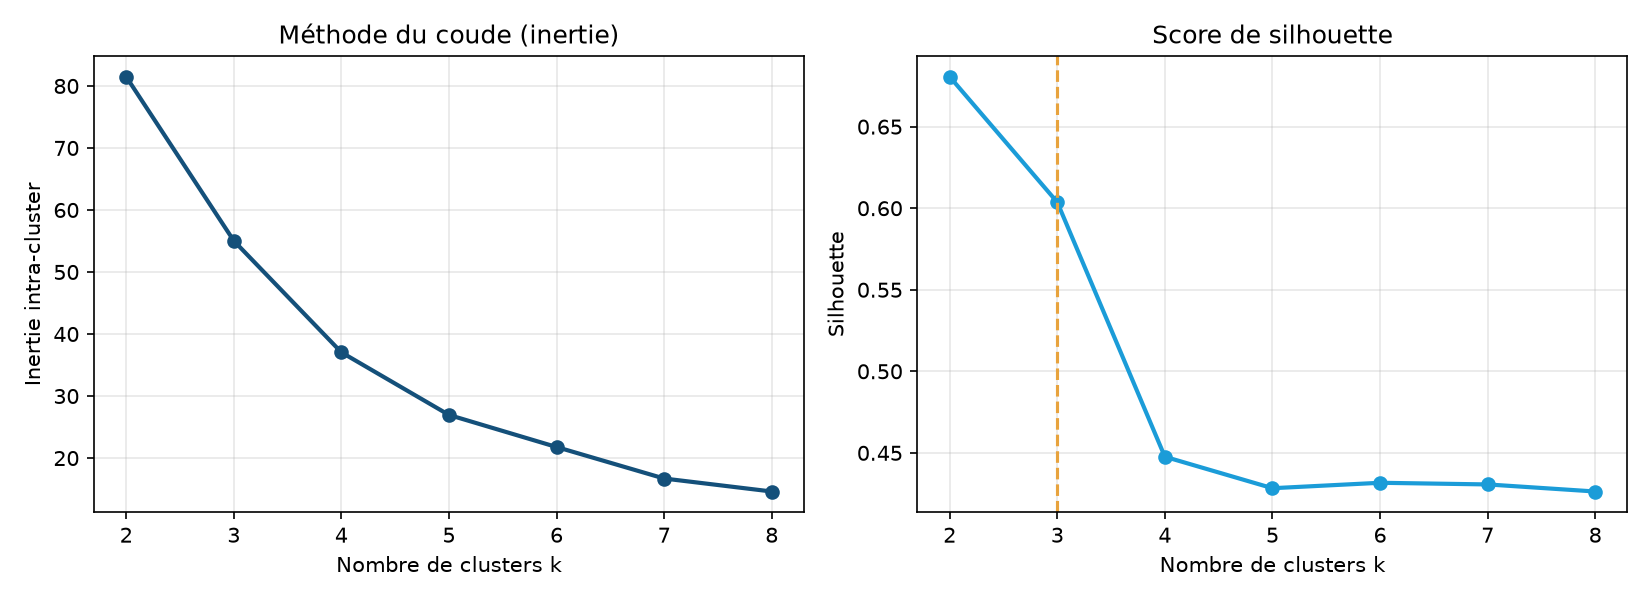
\includegraphics[width=\textwidth]{clustering_choix_k.png}
  \caption{Choix du nombre de clusters : méthode du coude et score de silhouette}
  \label{fig:choix_k}
\end{figure}

Les deux indicateurs concordent : l'inertie présente un \textbf{coude marqué à
$k=3$} et le score de silhouette y atteint son \textbf{maximum}
($\approx 0{,}74$). La segmentation en \textbf{trois clusters} est donc retenue.

\subsection{Comparaison des modèles de clustering}
Quatre algorithmes ont été comparés : \textbf{K-Means}, \textbf{classification
ascendante hiérarchique} (agglomératif), \textbf{modèle de mélange gaussien} (GMM)
et \textbf{DBSCAN}, à l'aide de trois indices internes
(tableau~\ref{tab:comparaison_clustering}, figure~\ref{fig:comparaison_clustering}).

\begin{table}[htbp]
\centering
\caption{Comparaison des modèles de clustering}
\label{tab:comparaison_clustering}
\renewcommand{\arraystretch}{1.25}
\begin{tabularx}{\textwidth}{>{\bfseries}lcccc}
\toprule
\textmd{\textbf{Modèle}} & \textbf{Nb clusters} & \textbf{Silhouette $\uparrow$} &
\textbf{Davies-Bouldin $\downarrow$} & \textbf{Calinski-Harabasz $\uparrow$}\\
\midrule
K-Means        & 3 & \textbf{0,736} & \textbf{0,350} & \textbf{391}\\
Agglomératif   & 3 & 0,736 & 0,350 & 391\\
GMM            & 3 & 0,736 & 0,350 & 391\\
DBSCAN         & 3 & 0,736 & 0,350 & 391\\
\bottomrule
\end{tabularx}
\end{table}

\begin{figure}[htbp]
  \centering
  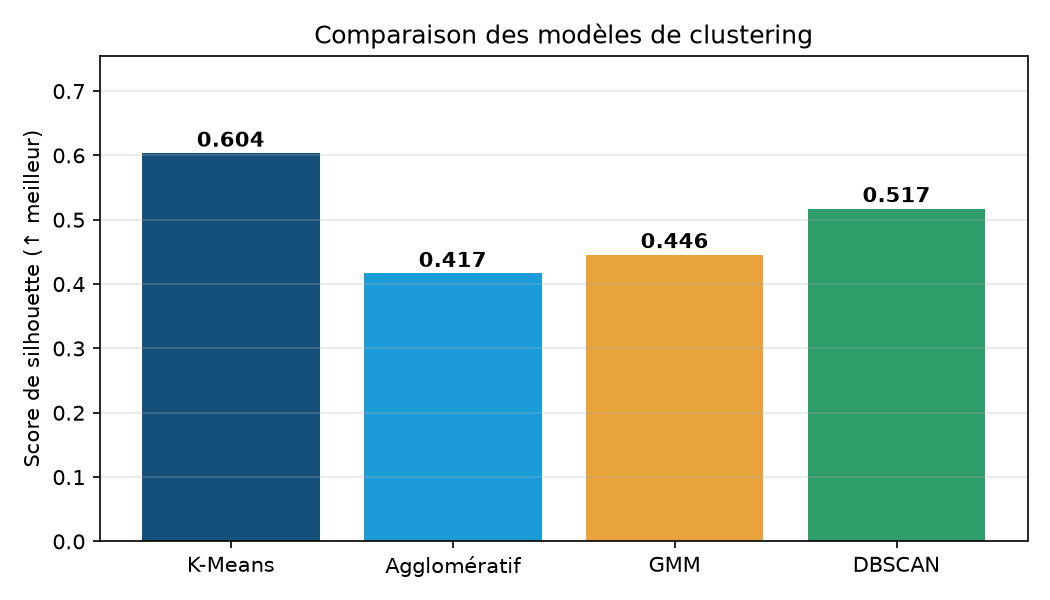
\includegraphics[width=0.7\textwidth]{clustering_comparaison.png}
  \caption{Comparaison des modèles selon le score de silhouette}
  \label{fig:comparaison_clustering}
\end{figure}

Les quatre algorithmes \textbf{convergent vers la même segmentation} : ils
identifient les trois mêmes clusters et obtiennent des indices identiques
(silhouette $0{,}736$, Davies-Bouldin $0{,}350$, Calinski-Harabasz $391$). Cette
concordance, y compris pour des approches de nature différente (partitionnement,
hiérarchique, probabiliste et à base de densité), confirme la \textbf{robustesse}
des trois segments. Le \textbf{K-Means} est retenu : il atteint le meilleur score
tout en restant simple et interprétable.

\section{Réalisation : résultats et interprétation}
La figure~\ref{fig:clusters_pca} projette les agences dans le plan des deux
premières composantes principales (PCA), colorées selon leur cluster ; la première
composante, qui résume la \emph{taille} de l'agence, explique l'essentiel de la
variance. Les trois segments sont nettement séparés.

\begin{figure}[htbp]
  \centering
  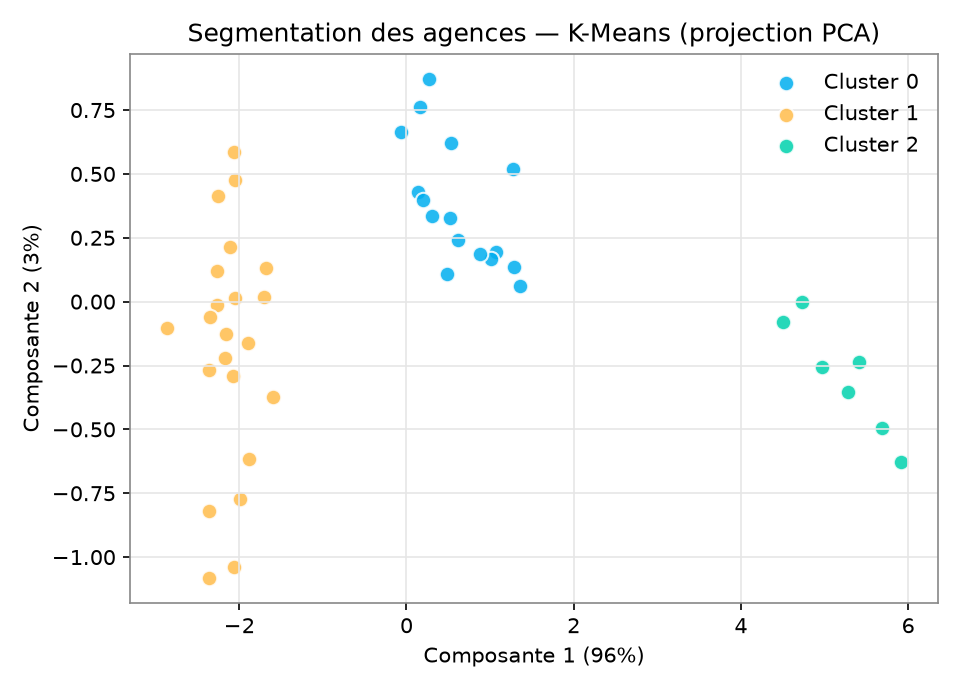
\includegraphics[width=0.78\textwidth]{clustering_pca.png}
  \caption{Segmentation des agences (K-Means) projetée par PCA}
  \label{fig:clusters_pca}
\end{figure}

Le profil moyen de chaque segment (tableau~\ref{tab:profils_clusters}) permet de
les caractériser.

\begin{table}[htbp]
\centering
\caption{Profil moyen des segments d'agences}
\label{tab:profils_clusters}
\renewcommand{\arraystretch}{1.25}
\begin{tabularx}{\textwidth}{>{\bfseries}Xcccccc}
\toprule
\textmd{\textbf{Segment}} & \textbf{Nb} & \textbf{Effectif} & \textbf{Clients} &
\textbf{Comptes} & \textbf{Prod. crédits} & \textbf{Présence}\\
\midrule
Grandes agences   & 7  & 116 & 908 & 2333 & 1734 & 0,98\\
Moyennes agences  & 16 & 54  & 438 & 1076 & 823  & 0,94\\
Petites agences   & 22 & 21  & 160 & 431  & 321  & 0,87\\
\bottomrule
\end{tabularx}
\end{table}

On distingue ainsi un segment de \textbf{grandes agences} (pôles majeurs à fort
effectif et forte production), un segment d'\textbf{agences moyennes} (activité
intermédiaire) et un segment de \textbf{petites agences} (effectif et activité
réduits, taux de présence plus faible).

\subsection{Apport décisionnel}
Cette segmentation constitue un outil d'\textbf{aide à la décision} : elle permet
d'adapter les actions à chaque profil --- allouer les ressources selon la taille,
fixer des objectifs différenciés, accompagner spécifiquement les petites agences
ou capitaliser sur les grandes. Elle prolonge le volet décisionnel et illustre
l'apport de l'\textbf{intelligence artificielle} au pilotage du réseau.

\section*{Conclusion}
Ce sprint a enrichi la solution d'une dimension analytique avancée. Après
détermination du nombre optimal de clusters et comparaison de plusieurs modèles,
le K-Means a fait émerger trois segments d'agences cohérents et exploitables pour
la décision.
             % Ch.8 — Sprint 6 : Segmentation
% ============================ CONCLUSION ==============================
\chapter*{Conclusion générale et perspectives}
\addcontentsline{toc}{chapter}{Conclusion générale et perspectives}
\markboth{CONCLUSION GÉNÉRALE}{}

Ce projet de fin d'études a permis de concevoir et de réaliser, au sein de la
\textbf{BTK -- Banque Tuniso-Koweïtienne}, une application web de gestion des
agences bancaires adossée à un volet décisionnel, conduite selon la méthodologie
\textbf{CRISP-DM}. La solution centralise la gestion des agences, des employés, des
clients et des objectifs, assure le \textbf{pointage} des employés, encadre les
opérations sensibles par des circuits de validation et restitue des indicateurs
d'aide à la décision via un tableau de bord et Power BI. Elle intègre en outre une
chaîne \textbf{ETL} et une brique d'\textbf{intelligence artificielle} : la
segmentation des agences par apprentissage non supervisé (clustering).

Ce travail a été l'occasion de mettre en pratique les compétences de la formation
--- modélisation UML, développement Jakarta EE, base de données Oracle, chaîne
décisionnelle (ETL en Python et \emph{reporting} Power BI) et initiation à
l'\textbf{apprentissage automatique} --- au croisement du développement logiciel
et de la Business Intelligence.

Plusieurs \textbf{difficultés} ont jalonné le projet et ont constitué autant
d'occasions d'apprentissage. La \textbf{consolidation} de données dispersées à des
grains hétérogènes a nécessité une chaîne ETL robuste et rejouable. L'articulation
entre le système opérationnel Oracle et l'outil de restitution Power BI a demandé
une attention particulière à la \textbf{modélisation décisionnelle} (schéma en
étoile, mesures) et à la préparation des données. Enfin, la mise au point de la
segmentation a exigé une démarche méthodique de choix et de comparaison de modèles
afin d'en garantir la robustesse. Ces défis ont renforcé une compétence clé :
\textbf{transformer une donnée brute en information utile à la décision}.

Plusieurs perspectives d'évolution peuvent être envisagées :
\begin{itemize}[noitemsep]
  \item le chiffrement (hachage) des mots de passe et le renforcement de la
        sécurité ;
  \item l'\textbf{industrialisation} de la chaîne ETL : ordonnancement automatique
        et historisation incrémentale des indicateurs ;
  \item l'enrichissement par des analyses prédictives (prévision des objectifs) ;
  \item l'exposition d'une API REST pour l'interopérabilité avec d'autres
        systèmes ;
  \item le développement d'une application mobile de consultation des indicateurs.
\end{itemize}
          % Conclusion générale

% ============================ NÉTOGRAPHIE =============================
\cleardoublepage
\renewcommand{\bibname}{Nétographie}
\addcontentsline{toc}{chapter}{Nétographie}
\nocite{*}
\bibliographystyle{ieeetr}
\bibliography{references}

% ============================ ANNEXES =================================
\cleardoublepage
\appendix
% ============================ ANNEXES =================================
\chapter{Annexes}

Cette annexe rassemble des extraits du code réel du projet : la chaîne ETL, la
segmentation par apprentissage automatique et une vue décisionnelle SQL.

% ---------------------------------------------------------------------
\section{Chaîne ETL --- extraction, transformation, chargement (Python)}
Extraits du script \texttt{etl/etl\_agences.py}. La fonction \texttt{extract\_oracle}
lit les tables opérationnelles ; \texttt{transform} agrège les indicateurs par
agence ; \texttt{load} écrit le datamart en étoile.

\begin{lstlisting}[style=pycode,language=Python,caption={Extraction des sources depuis Oracle}]
def extract_oracle(dsn=None, user=None, password=None):
    import oracledb
    cn = oracledb.connect(
        user=user or os.environ.get("BTK_DB_USER", "system"),
        password=password or os.environ.get("BTK_DB_PWD", ""),
        dsn=dsn or os.environ.get("BTK_DB_DSN", "localhost:1521/FREEPDB1"))
    ag  = pd.read_sql("SELECT SK_AGENCE, LIBELLE_AGENCE, DISTRICT FROM AGENCE", cn)
    emp = pd.read_sql("SELECT SK_UTILISATEUR, SK_AGENCE, EST_GESTIONNAIRE "
                      "FROM B_UTILISATEURS", cn)
    cli = pd.read_sql("SELECT SK_CLIENT, SK_AGENCE FROM CLIENT_BTK", cn)
    obj = pd.read_sql(
        "SELECT SK_AGENCE, "
        "  NVL(SOUSCRIPTION_COMPTE_CHEQUES_OA,0)+NVL(SOUSCRIPTION_COMPTE_EPARGNES_OA,0)"
        "  +NVL(SOUSCRIPTION_COMPTE_COURANTS_OA,0) AS COMPTES, "
        "  NVL(PRODUCTION_CREDITS_CONSO_OA,0)+NVL(PRODUCTION_CREDITS_IMMO_OA,0)"
        "  +NVL(PRODUCTION_CREDITS_INVESTISSEMENT_OA,0) AS CREDITS, "
        "  NVL(EPARGNE_ADD_OA,0) AS EPARGNE FROM B_OBJECTIF", cn)
    poi = pd.read_sql("SELECT P.SK_UTILISATEUR, U.SK_AGENCE, P.STATUT "
                      "FROM POINTAGE P JOIN B_UTILISATEURS U "
                      "ON P.SK_UTILISATEUR = U.SK_UTILISATEUR", cn)
    cn.close()
    return ag, emp, cli, obj, poi
\end{lstlisting}

\begin{lstlisting}[style=pycode,language=Python,caption={Transformation (agrégation par agence) et chargement du datamart}]
def transform(agences, employes, clients, objectifs, pointages):
    eff = employes.groupby("SK_AGENCE").agg(
        effectif=("SK_UTILISATEUR", "count"),
        nb_gestionnaires=("EST_GESTIONNAIRE", "sum")).reset_index()
    cli = clients.groupby("SK_AGENCE").size().reset_index(name="nb_clients")
    obj = objectifs.groupby("SK_AGENCE").agg(
        total_comptes=("COMPTES", "sum"),
        production_credits=("CREDITS", "sum"),
        collecte_epargne=("EPARGNE", "sum")).reset_index()
    poi = pointages.assign(
            present=pointages["STATUT"].isin(["PRESENT", "RETARD"]).astype(int)) \
        .groupby("SK_AGENCE").agg(taux_presence=("present", "mean")).reset_index()
    dm = agences.merge(eff, on="SK_AGENCE", how="left") \
                .merge(cli, on="SK_AGENCE", how="left") \
                .merge(obj, on="SK_AGENCE", how="left") \
                .merge(poi, on="SK_AGENCE", how="left")
    return dm.rename(columns={"LIBELLE_AGENCE": "agence"})

def load(dm):
    dim_agence  = dm[["SK_AGENCE", "agence", "DISTRICT"]]
    fait_agence = dm[["SK_AGENCE"] + FEATURES]
    dim_agence.to_csv(os.path.join(ENTREPOT, "dim_agence.csv"), index=False)
    fait_agence.to_csv(os.path.join(ENTREPOT, "fait_agence.csv"), index=False)
    dm[["agence"] + FEATURES].to_csv(DATAMART, index=False)
\end{lstlisting}

% ---------------------------------------------------------------------
\section{Segmentation des agences (Python, scikit-learn)}
Extraits du script \texttt{clustering/segmentation\_agences.py} : la standardisation
des variables et la détermination du nombre optimal de clusters (méthode du coude
combinée au score de silhouette).

\begin{lstlisting}[style=pycode,language=Python,caption={Choix du nombre de clusters (coude + silhouette)}]
from sklearn.preprocessing import StandardScaler
from sklearn.cluster import KMeans
from sklearn.metrics import silhouette_score

X = StandardScaler().fit_transform(df[FEATURES])   # centrage-reduction

def choisir_k(X, kmax=8):
    ks = list(range(2, kmax + 1))
    inerties, silhouettes = [], []
    for k in ks:
        km = KMeans(n_clusters=k, n_init=10, random_state=42).fit(X)
        inerties.append(km.inertia_)                # methode du coude
        silhouettes.append(silhouette_score(X, km.labels_))
    return ks[int(np.argmax(silhouettes))]          # k au meilleur silhouette
\end{lstlisting}

\begin{lstlisting}[style=pycode,language=Python,caption={Comparaison des modèles et profilage des segments}]
modeles = {
    "K-Means":      KMeans(n_clusters=k, n_init=10, random_state=42),
    "Agglomeratif": AgglomerativeClustering(n_clusters=k),
    "GMM":          GaussianMixture(n_components=k, random_state=42),
    "DBSCAN":       DBSCAN(eps=1.2, min_samples=3),
}
for nom, modele in modeles.items():
    labels = modele.fit_predict(X)
    sil = silhouette_score(X, labels)
    db  = davies_bouldin_score(X, labels)
    ch  = calinski_harabasz_score(X, labels)
    print(nom, round(sil, 3), round(db, 3), round(ch))
# profil moyen de chaque segment
df["cluster"] = KMeans(n_clusters=k, n_init=10, random_state=42).fit_predict(X)
profils = df.groupby("cluster")[FEATURES].mean()
\end{lstlisting}

% ---------------------------------------------------------------------
\section{Vue décisionnelle (SQL)}
Exemple de vue analytique exposée à Power BI (\texttt{sql/v\_bi\_employes.sql}) :
elle joint les employés à leur agence et calcule le rôle métier.

\begin{lstlisting}[style=pycode,language=SQL,caption={Vue décisionnelle V\_BI\_EMPLOYES}]
CREATE OR REPLACE VIEW V_BI_EMPLOYES AS
SELECT
    U.SK_UTILISATEUR       AS ID_EMPLOYE,
    U.LIBELLE_UTILISATEUR  AS NOM_COMPLET,
    U.EMAIL_UTILISATEUR    AS EMAIL,
    CASE
        WHEN U.EST_GESTIONNAIRE = 1 THEN 'Gestionnaire'
        WHEN U.EST_GESTIONNAIRE = 0 AND U.SK_AGENCE = 31 THEN 'Hors Commercial'
        ELSE 'Conseiller'
    END AS ROLE_LABEL,
    CASE WHEN U.EST_SUSPENDU = 1 THEN 'Suspendu' ELSE 'Actif' END AS STATUT,
    A.LIBELLE_AGENCE AS NOM_AGENCE,
    A.DISTRICT       AS DISTRICT_AGENCE
FROM B_UTILISATEURS U
LEFT JOIN AGENCE A ON U.SK_AGENCE = A.SK_AGENCE;
\end{lstlisting}

% ---------------------------------------------------------------------
\section{Dépôt du code source}
Le code source complet du projet --- application Jakarta EE (entités, servlets,
services, pages JSP), scripts SQL d'initialisation, chaîne ETL et segmentation
Python, thème et modèle Power BI --- est versionné sur le dépôt Git associé à ce
rapport.


\end{document}
